\chapter{Diseño del sistema multi-USV cooperativo}
\label{cap:diseno}

Este capítulo desarrolla la rama izquierda del Modelo en V definida en la Sección~\ref{subsec:modelo_v}. El 
punto de partida es el diagnóstico de la plataforma del Apéndice~\ref{ap:diagnostico}, que identifica los 
subsistemas que deben incorporarse o desarrollarse. A partir de los requisitos del sistema, constituidos por 
el concepto ganador de la Tabla~\ref{tab:concepto_ganador} y por las 
métricas de la Tabla~\ref{tab:metricas}, y desciende hacia la arquitectura del sistema, el diseño detallado de 
cada subsistema y su implementación. Puesto que la selección de cada componente ya se justificó en la 
Sección~\ref{sec:seleccion_concepto}, aquí no se discute qué componente se emplea, sino cómo se integran los 
componentes seleccionados para formar un sistema operativo. Cada decisión de diseño se vincula con la métrica 
que atiende y, a través de esta, con la prueba respectiva de la Sección~\ref{sec:pruebas}.
 
% ---------------------------------------------------------------------
\section{Arquitectura general del sistema}
\label{sec:arquitectura_general}
 
El sistema se compone de tres nodos físicos: una estación base en tierra y dos vehículos de superficie, USV1 y 
USV2, construidos sobre las plataformas Invader descritas en la Sección~\ref{subsec:invader}. La estación base 
supervisa la misión y coordina la flota, y cada USV ejecuta de forma autónoma las consignas que recibe. Esta 
sección presenta la composición de la flota, los flujos de información y control, el algoritmo de operación y las 
limitaciones de la arquitectura; el diseño detallado de cada subsistema se aborda en las secciones siguientes.
 
% ---------------------------------------------------------------------
\subsection{Composición heterogénea de la flota}
\label{subsec:flota_heterogenea}
 
La flota es heterogénea y con roles diferenciados. El USV1 actúa como vehículo líder: además del autopiloto 
Pixhawk~6X, integra el ordenador a bordo Jetson Orin Nano y la cámara USB, con los que percibe el entorno, 
detecta obstáculos y registra la información visual de la misión. El USV2 actúa como vehículo seguidor e integra 
el autopiloto, los sensores de navegación, el módulo de medición de potencia y los equipos de comunicación, sin 
ordenador a bordo ni cámara. Ambos mantienen la propulsión y la estructura de la plataforma original (SF9 y SF10).
 
Esta asimetría responde a la jerarquía de necesidades de la Tabla~\ref{tab:necesidades}: la coordinación de dos 
USV es imprescindible y exige que ambos naveguen de forma autónoma, mientras que la captura de imágenes, de 
importancia 3, puede demostrarse con un único vehículo. Omitir el ordenador a bordo y la cámara en el USV2 reduce 
la masa añadida y su efecto sobre la estabilidad (M7 y M11) sin renunciar a la percepción en la flota, ya que, 
mediante el esquema líder--seguidor descrito en la Sección~\ref{subsec:concepto_operacion}, el USV2 solo navega 
por la trayectoria que el USV1 ya ha inspeccionado. Además, la configuración demuestra que un vehículo que solo 
disponga de autopiloto y enlace de red puede incorporarse a la flota sin modificar la lógica de la estación base, 
lo que facilita la extensión futura a más vehículos. La Tabla~\ref{tab:distribucion_subfunciones} resume el reparto 
de las subfunciones entre los tres nodos.
 
\begin{table}[!htb]
\centering
\caption{Distribución de las subfunciones del sistema entre la estación base y los dos USV.}
\label{tab:distribucion_subfunciones}
\footnotesize
\renewcommand{\arraystretch}{1.15}
\begin{tabularx}{\textwidth}{|>{\raggedright\arraybackslash}p{3.7cm}|>{\raggedright\arraybackslash}X|>{\raggedright\arraybackslash}X|>{\raggedright\arraybackslash}X|}
\hline
\textbf{Subfunción} & \textbf{Estación base} & \textbf{USV1 (líder)} & \textbf{USV2 (seguidor)} \\ \hline
SF1 Recibir y ejecutar comandos & -- & Pixhawk 6X con GNSS M8N & Pixhawk 6X con GNSS M8N \\ \hline
SF2 Procesar datos de alto nivel & -- & Jetson Orin Nano 8 GB & -- \\ \hline
SF3 Percibir el entorno & -- & Cámara USB & -- \\ \hline
SF4 Almacenar y registrar datos & rosbag2 de ambos USV & Registro del autopiloto (rosbag2 local opcional) & Registro del 
autopiloto \\ \hline
SF5 Medir consumo de energía & -- & I2C-INA-BM & I2C-INA-BM \\ \hline
SF6 Almacenar y distribuir energía & -- & TATTU 6S (autopiloto, Jetson y Bullet AC) & TATTU 6S (autopiloto y Bullet AC) \\ \hline
SF7 Transmitir por radiofrecuencia & RFD900x & RFD900x & RFD900x \\ \hline
SF8 Transmitir por red local & Rocket Prism 5AC Gen2 (punto de acceso) & Bullet AC (estación) & Bullet AC 
(estación) \\ \hline
SF9 Dar propulsión & -- & Propulsión existente & Propulsión existente \\ \hline
SF10 Integrar y proteger la estructura & -- & Casco existente & Casco existente \\ \hline
\end{tabularx}
\end{table}
 
En el USV2, que carece de ordenador a bordo, el registro de datos (SF4) se resuelve combinando los registros 
internos de su autopiloto con la grabación que la estación base realiza de los tópicos de ambos vehículos, de 
modo que la trayectoria, las señales de control y el consumo de los dos USV quedan registrados. El hardware 
nuevo se alimenta desde una batería independiente de la propulsión (SF6), cuya distribución se detalla en la 
Sección~\ref{subsec:alimentacion}.
 
\newpage
\FloatBarrier

% ---------------------------------------------------------------------
\subsection{Arquitectura de información y control}
\label{subsec:arquitectura_informacion}
 
El control se organiza en tres niveles, representados en la Figura~\ref{fig:arquitectura_informacion}. En la 
estación base, un nodo coordinador de ROS~2 define la misión, asigna los \textit{waypoints} y sigue el progreso 
de la flota, mientras el operador supervisa ambos vehículos desde la estación de control y los datos de la misión 
se registran. En el USV1, el ordenador a bordo ejecuta ROS~2 Jazzy y se encarga de la percepción y del registro 
de imágenes. En ambos vehículos, el autopiloto con ArduPilot Rover estima el estado, calcula las consignas de 
rumbo y velocidad, gobierna los propulsores y ejecuta los mecanismos de seguridad \cite{kumar2025} \cite{aliane2026}.

\FloatBarrier
\begin{figure}[htbp]
\centering
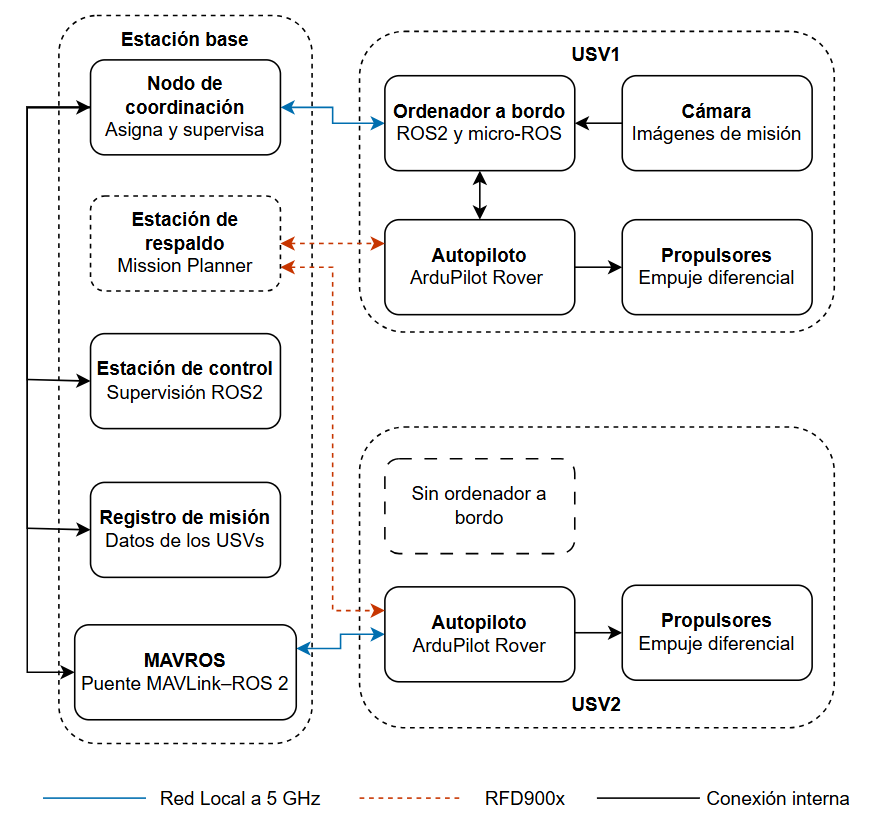
\includegraphics[width=0.95\textwidth]{fig/arquitectura_funcional.png}
\caption{Arquitectura de información y control del sistema multi-USV.}
\label{fig:arquitectura_informacion}
\end{figure}
 
La heterogeneidad de la flota da lugar a dos caminos de comunicación que convergen en un mismo grafo de ROS~2. En 
el USV1, el autopiloto se conecta por un enlace serie al ordenador a bordo y publica sus datos como tópicos de 
ROS~2 mediante la interfaz DDS nativa de ArduPilot y el agente micro-ROS de la Jetson; estos tópicos alcanzan la 
estación base a través del enlace Ubiquiti gracias al descubrimiento descentralizado de DDS \cite{albatati2026}. 
En el USV2, el autopiloto se conecta por Ethernet al radio Bullet AC y envía MAVLink sobre UDP a la estación base, 
donde MAVROS lo traduce a tópicos de ROS~2. Al publicar cada vehículo bajo su propio espacio de nombres, 
\texttt{/usv1} y \texttt{/usv2}, el coordinador interactúa con ambos de la misma forma.
 
Sobre esta estructura se apoya la cooperación. El USV1 publica su posición y, si detecta un obstáculo, este genera un aviso; 
el coordinador traduce ambos en consignas para el USV2, al que envía a través de MAVROS los puntos de la 
trayectoria del líder o la orden de detenerse. Para ello, el autopiloto del USV2 opera en modo Guided 
(Sección~\ref{subsec:mavlink_mavros}). Como la comunicación sigue una topología en estrella, todo intercambio 
entre vehículos atraviesa la estación base, y la latencia entre ellos es aproximadamente la suma de las de cada 
uno con la base (Sección~\ref{subsec:metricas_enlace}); por ello, M5 se mide entre la base y cada USV.
 
La red local es la fuente principal de telemetría, que el operador supervisa con herramientas de ROS~2. 
En paralelo, el radiomódem RFD900x de cada autopiloto mantiene activa la telemetría MAVLink hacia una estación de 
respaldo con Mission Planner \cite{iniesta2025}, y el receptor de radiocontrol permite recuperar el control manual 
en cualquier momento. Así, la pérdida de la red local no implica la pérdida de la supervisión ni del control de 
los vehículos. El diseño de ambos enlaces se detalla en la Sección~\ref{sec:diseno_comunicaciones}.
 
% ---------------------------------------------------------------------
\subsection{Concepto de operación}
\label{subsec:concepto_operacion}
 
El algoritmo de operación se representa, con independencia de los componentes, en dos figuras unidas por los 
conectores A y B: la Figura~\ref{fig:flujo_prep_cierre} recoge la preparación y el cierre de la misión, comunes a 
toda la flota, y la Figura~\ref{fig:flujo_ejecucion}, la ejecución cooperativa.

\begin{figure}[!htb]
\centering
\begin{subfigure}[t]{0.48\textwidth}
  \centering
  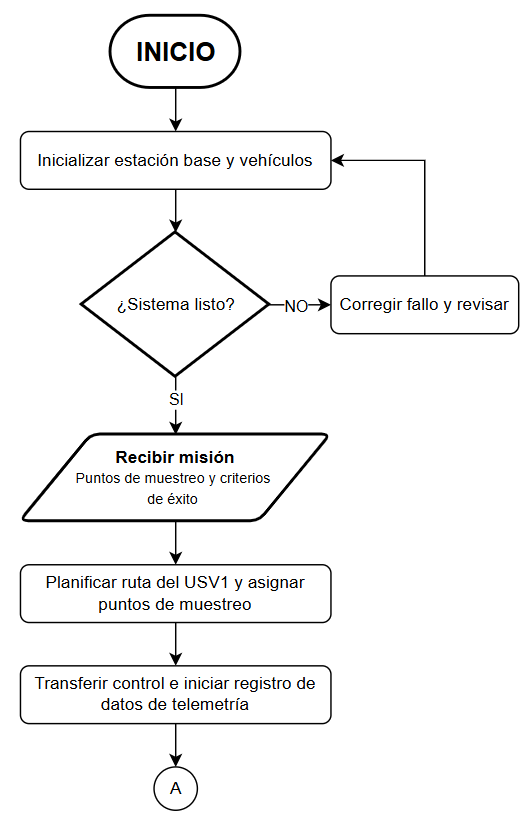
\includegraphics[width=\textwidth]{fig/flujo_inicio.png}
  \caption{Preparación de la misión}
  \label{fig:flujo_preparacion}
\end{subfigure}\hfill
\begin{subfigure}[t]{0.48\textwidth}
  \centering
  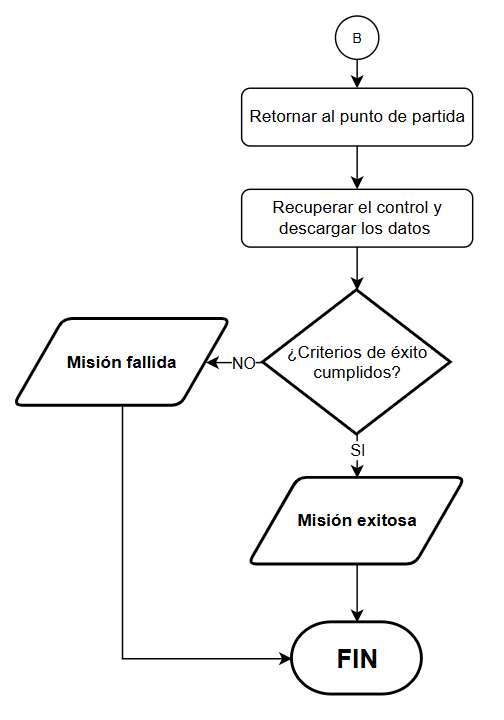
\includegraphics[width=\textwidth]{fig/flujo_fin.png}
  \caption{Cierre de la misión}
  \label{fig:flujo_cierre}
\end{subfigure}
\caption{Fases de preparación y cierre del algoritmo de operación}
\label{fig:flujo_prep_cierre}
\end{figure}
 
En la preparación (Figura~\ref{fig:flujo_preparacion}), el sistema verifica los enlaces y el autodiagnóstico de 
cada vehículo antes de continuar, de modo que ninguna misión comienza con un vehículo no apto. El operador 
introduce los puntos de muestreo y los criterios de éxito de la misión, el coordinador carga la ruta en el 
USV1 y prepara la del USV2, que recorre los mismos puntos y, al transferir el control al sistema autónomo, se 
inicia el registro de datos.


\begin{figure}[!htb]
\centering
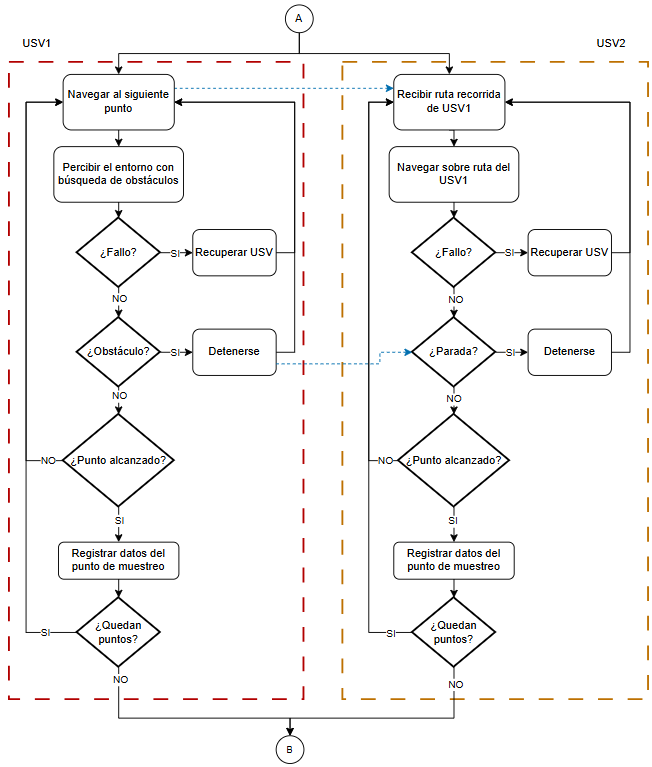
\includegraphics[width=\textwidth,height=0.95\textheight,keepaspectratio]{fig/flujo_cooperativo.png}
\caption{Ejecución cooperativa de la misión con el esquema líder--seguidor.}
\label{fig:flujo_ejecucion}
\end{figure}
 
En la ejecución (Figura~\ref{fig:flujo_ejecucion}), ambos vehículos navegan de forma simultánea sobre 
la misma ruta, el USV2 con retraso respecto al líder. El 
USV1 navega hacia cada punto de su ruta mientras percibe el entorno: ante un fallo propio, como la pérdida de 
un enlace, la falta de energía o la degradación del posicionamiento, ejecuta el subproceso de recuperación, y 
ante un obstáculo se detiene y el aviso se transmite al USV2 a través de la base. El USV2 recibe la ruta ya 
recorrida por el líder y navega sobre ella con una distancia de separación; conserva la misma comprobación de 
fallos, que realiza su autopiloto, pero sustituye la detección de obstáculos por la comprobación de una orden de 
parada. Ambos registran los datos al entrar en el círculo de aceptación de cada punto de muestreo \cite{jin2025}. 
La cooperación consiste así en compartir la percepción: el USV2 solo avanza por zonas inspeccionadas por el USV1 
y, si deja de recibir una ruta actualizada, permanece detenido. La fase termina cuando los dos vehículos han 
completado sus puntos.
 
En el cierre (Figura~\ref{fig:flujo_cierre}), los vehículos retornan al punto de partida, se descargan los 
registros y la misión se evalúa frente a los criterios definidos en la preparación, clasificándose como exitosa 
o fallida. Además, cada punto de muestreo alcanzado o no alcanzado durante la misión constituye uno de los ensayos 
con los que se calcula la tasa de éxito de misión (M6), según lo definido en la Sección~\ref{sec:pruebas}.


% ---------------------------------------------------------------------
\subsection{Alcances y limitaciones de la arquitectura}
\label{subsec:alcances_arquitectura}
 
La arquitectura asume de forma deliberada cinco limitaciones. La estación base es el único punto de coordinación 
de la flota, consecuencia de la topología en estrella, adecuada para dos vehículos que operan dentro del alcance 
definido por M8. El USV2 depende del avance del líder y del enlace: si el USV1 se detiene o el enlace se pierde, 
permanece detenido, lo que sacrifica disponibilidad a cambio de seguridad. La detección de obstáculos se limita al 
campo de visión de la cámara del USV1, por lo que no se detectan los obstáculos que aparezcan tras su paso. Además, la 
georreferenciación absoluta de los datos depende del receptor GNSS estándar de cada autopiloto, con una 
incertidumbre del orden de 2~m \cite{Cite29}, suficiente para la navegación por \textit{waypoints} pero no para 
ubicar las muestras con precisión centimétrica. Por último, la información visual de la misión procede únicamente 
del USV1.
 
\newpage
\FloatBarrier
 
% =====================================================================
% Capítulo 4 — Sección 4.2: Arquitectura de comunicaciones (versión 2)
% Coherente con la 4.1 v4: supervisión en ROS 2, estación de respaldo con
% Mission Planner, esquema líder--seguidor.
% Claves \cite{...} provisionales -> ajustar a las de tu .bib:
%   gogendeau2024 [11], sears2024 [14], albatati2026 [21],
%   rfd900x [24], ubiquiti_ptmp [25], cnaf (NUEVA, entrada al final)
% Etiquetas: subsec:pruebas_integracion -> tu Sección 3.4.2
% =====================================================================

\section{Arquitectura de comunicaciones}
\label{sec:diseno_comunicaciones}
 
La arquitectura de comunicaciones materializa las subfunciones SF7 y SF8 y responde a la necesidad de 
mantener una comunicación confiable y de suficiente alcance entre los USV y la estación base, con un canal 
principal de tipo WiFi y un enlace de radio como canal redundante (Tabla~\ref{tab:necesidades}). Sus 
requisitos cuantitativos son la latencia de comunicación (M5), con un valor marginal de 1~s, y el alcance 
del enlace (M8), con un valor marginal de 100~m y un valor ideal de 1000~m. El diseño se divide en el 
enlace principal, basado en una red local Ubiquiti airMAX en la banda de 5~GHz; el plan de direccionamiento 
de esa red; y el enlace redundante, basado en los radiomódems RFD900x. La Figura~\ref{fig:arquitectura_comunicaciones} 
representa la arquitectura de comunicaciones completa.

\begin{figure}[!htb]
\centering
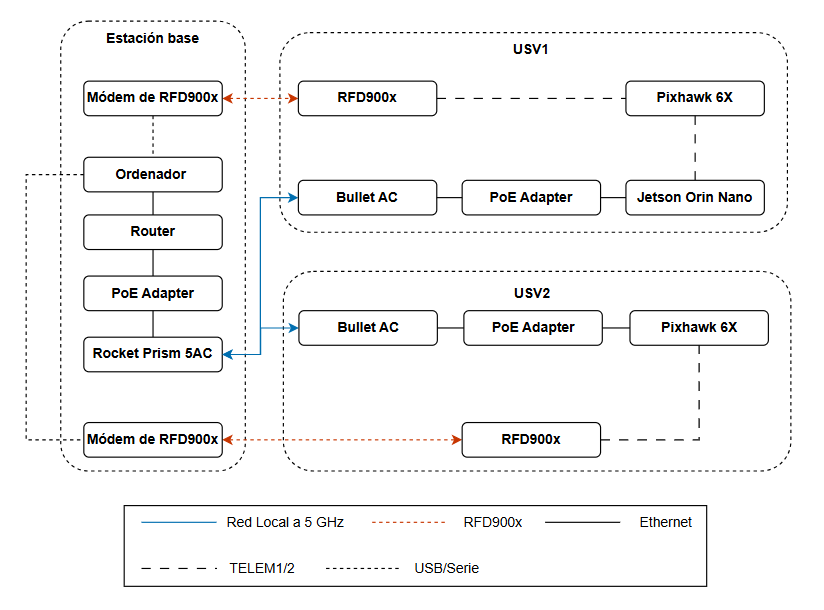
\includegraphics[width=1\textwidth]{fig/arquitectura_comunicaciones.png}
\caption{Arquitectura de comunicaciones del sistema multi-USV.}
\label{fig:arquitectura_comunicaciones}
\end{figure}
 
% ---------------------------------------------------------------------
\subsection{Enlace principal: red local airMAX en estrella}
\label{subsec:enlace_principal}
 
El enlace principal se organiza como una red punto a multipunto. El radio Rocket Prism 5AC Gen2 de la estación 
base opera como punto de acceso y cada USV incorpora un radio Bullet AC configurado como estación, con el mismo 
identificador de red, cifrado WPA2 con clave compartida y el dominio regulatorio de España en los tres 
equipos \cite{Cite25}. En la base, el Rocket se conecta mediante su inyector PoE al router, al que el 
equipo de la estación base se conecta por Ethernet. En cada vehículo, el puerto de datos del inyector PoE del 
Bullet se conecta al equipo que da acceso al vehículo: la Jetson Orin Nano en el USV1 y el puerto Ethernet del 
Pixhawk~6X en el USV2.

\newpage

La Figura~\ref{fig:equipos_red} muestra los dos radios empleados. Ambos disponen de conectores para antenas 
externas: el Rocket Prism admite dos antenas, una por cada cadena de radio, y el Bullet AC una, a través de 
su conector de tipo N y un adaptador para la antena SpiroNET.

\begin{figure}[!htb]
\centering
\begin{subfigure}[b]{0.45\textwidth}
  \centering
  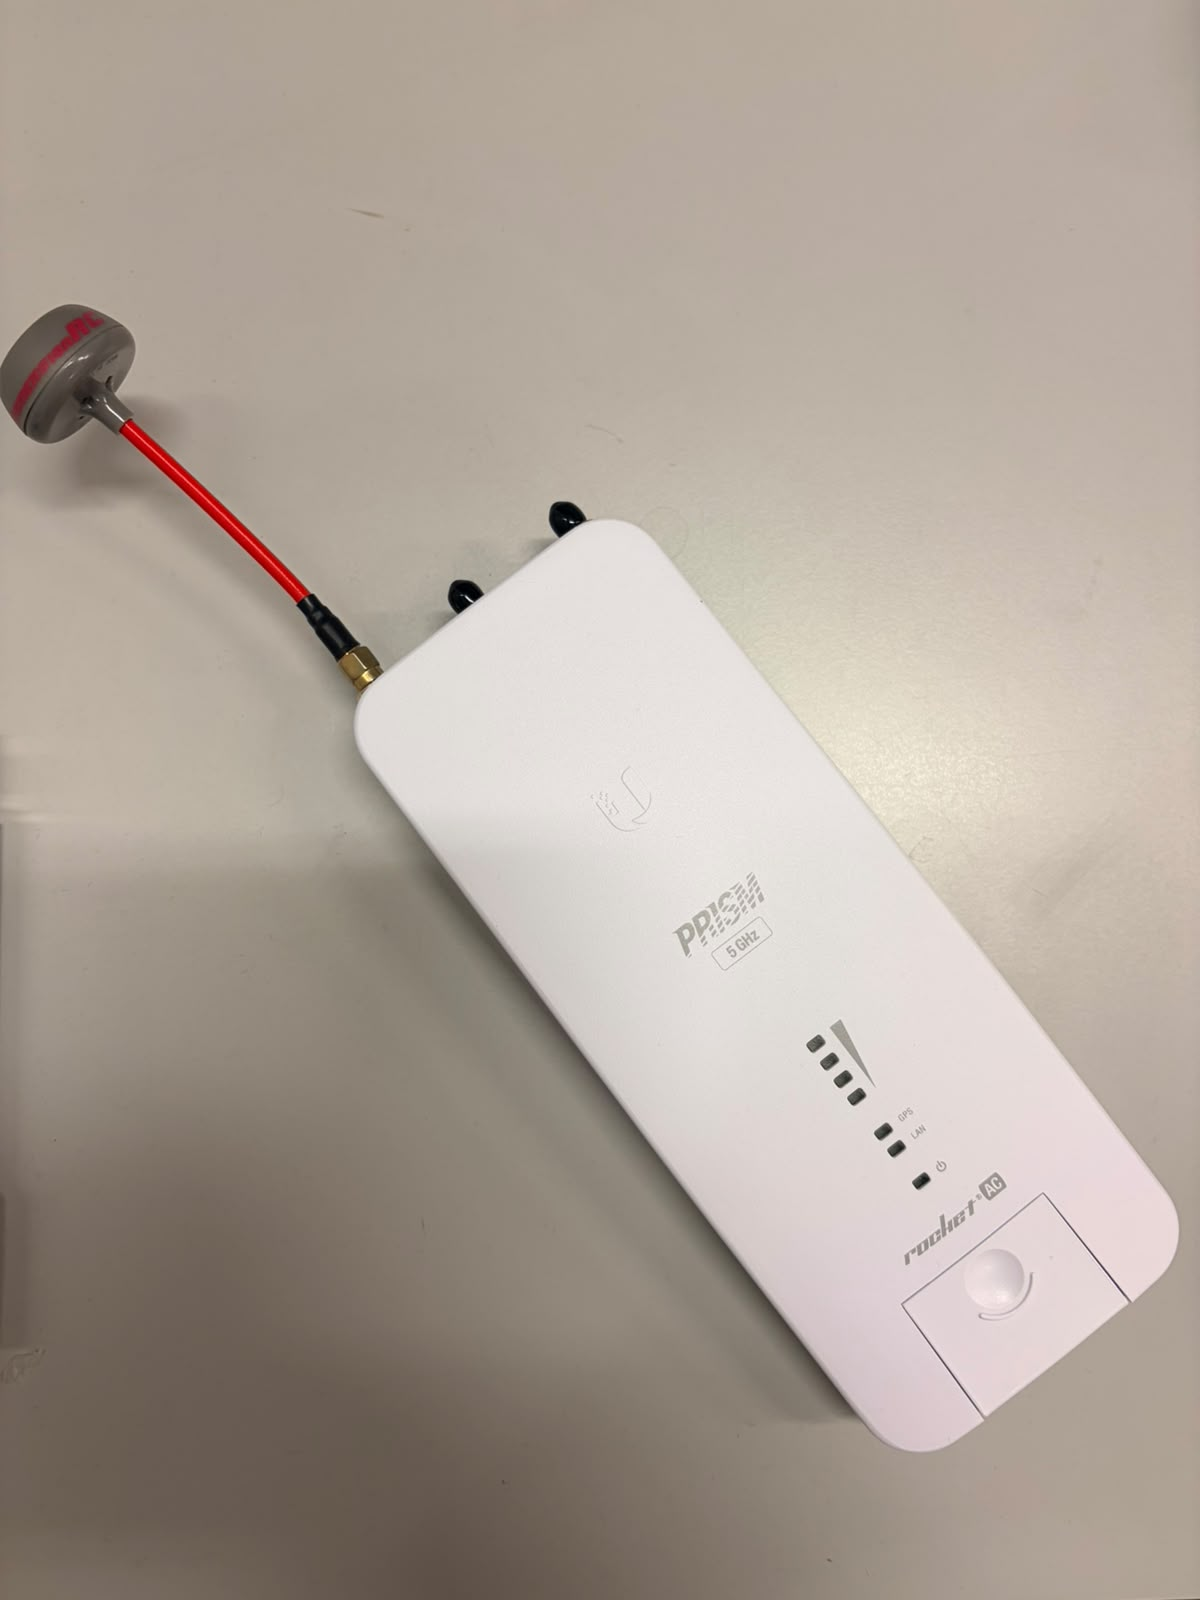
\includegraphics[height=7cm,keepaspectratio]{fig/rocket.jpeg}
  \caption{Rocket Prism 5AC Gen2 de la estación base, con una antena SpiroNET.}
  \label{fig:rocket}
\end{subfigure}\hfill
\begin{subfigure}[b]{0.45\textwidth}
  \centering
  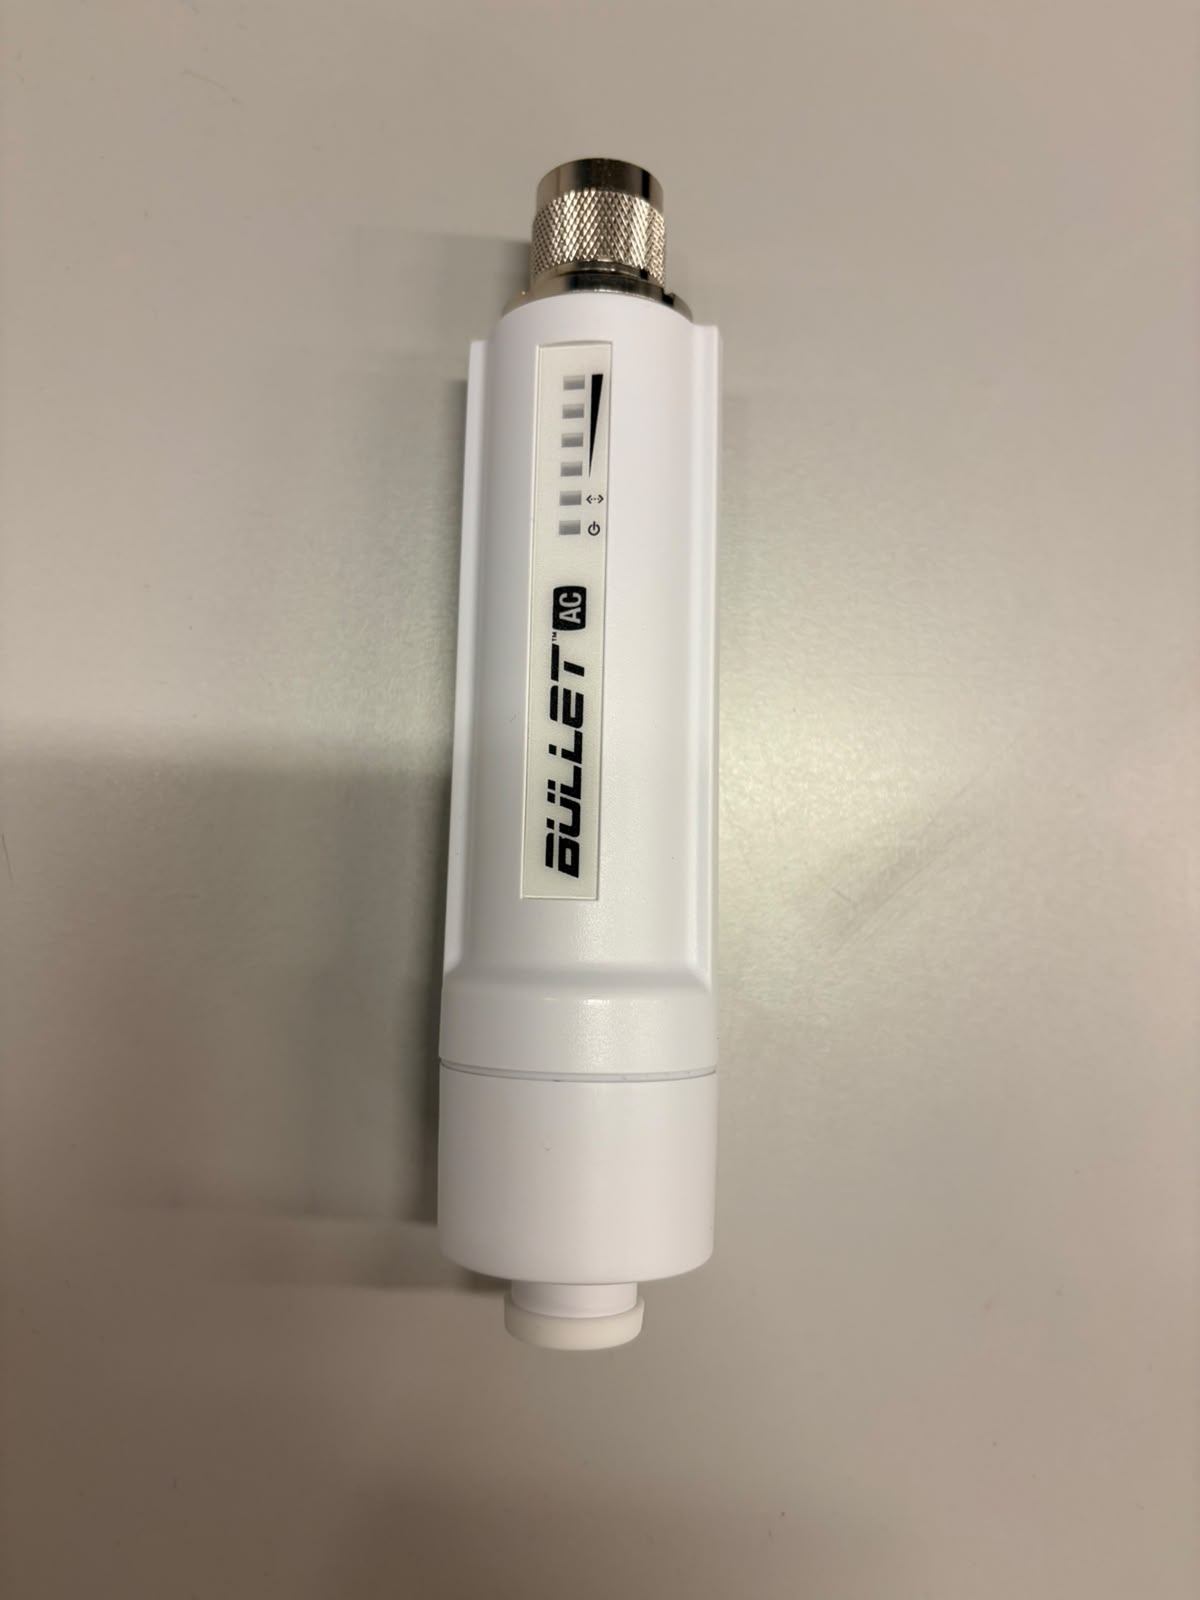
\includegraphics[height=7cm,keepaspectratio]{fig/bullet.jpeg}
  \caption{Bullet AC de los vehículos.}
  \label{fig:bullet}
\end{subfigure}
\caption{Radios de la red local empleados en el sistema.}
\label{fig:equipos_red}
\end{figure}
 
Los tres radios operan en modo puente transparente de capa~2, de modo que todos los equipos de la base y de 
los vehículos pertenecen a una misma subred, como si estuvieran conectados a un único conmutador. Esta elección 
simplifica la integración en dos aspectos: el descubrimiento de nodos de DDS, basado en mensajes de multidifusión, 
alcanza de forma nativa a la Jetson y al equipo de la base sin configurar encaminamiento alguno 
\cite{albatati2026}, y los mensajes MAVLink del USV2 viajan sobre UDP directamente entre su autopiloto y la 
instancia de MAVROS de la base. Además, el punto de acceso coordina el acceso al medio de las estaciones 
mediante el protocolo airMAX \cite{Cite25}, lo que resulta relevante en la flota, porque los dos USV 
pueden encontrarse lo bastante alejados como para no detectarse entre sí y, en un acceso por contienda, 
pueden transmitir simultáneamente hacia la base.
 
\subsubsection{Banda y canal de operación}
 
Las pruebas de banco y de laboratorio se realizan en el canal de 5210~MHz, perteneciente a la subbanda de 
5150--5250~MHz, que no exige selección dinámica de frecuencia (DFS) y permite establecer el enlace de forma 
inmediata. Sin embargo, de acuerdo con la nota UN-128 del Cuadro Nacional de Atribución de Frecuencias, las 
subbandas de 5150--5250~MHz y 5250--5350~MHz se restringen al uso en interiores, mientras que la de 
5470--5725~MHz admite el uso en exteriores con una potencia isótropa radiada equivalente (p.i.r.e.) máxima de 
1~W, siempre que el equipo emplee control de potencia y DFS \cite{cnaf}. Por ello, para la operación en cuerpos 
de agua el canal se traslada a la subbanda de 5470--5725~MHz, excluyendo el tramo de 5600--5650~MHz, reservado 
a radares meteorológicos.
 
El uso de DFS en exteriores tiene dos consecuencias que el diseño incorpora. Al arrancar, el punto de acceso 
verifica durante un tiempo que el canal está libre de radares antes de transmitir, por lo que esa espera forma 
parte de la fase de inicialización del sistema y no debe interpretarse como un fallo del enlace. Si durante la 
operación detecta un radar, abandona el canal y continúa en otro; para que las estaciones lo sigan sin 
intervención manual, los Bullet AC se configuran con el ancho de canal en modo automático y con una lista de 
exploración limitada a los canales permitidos.
 
\subsubsection{Ancho de canal}
 
El ancho de canal se dimensiona a partir del tráfico que debe soportar el enlace. La Tabla~\ref{tab:demanda_trafico} 
estima esa demanda para los dos vehículos, considerando que solo el USV1 transmite imágenes.
 
\begin{table}[!htb]
\centering
\caption{Estimación de la demanda de tráfico del enlace principal.}
\label{tab:demanda_trafico}
\small
\begin{tabular}{|p{5.2cm}|p{3.8cm}|p{4.8cm}|}
\hline
\textbf{Flujo de datos} & \textbf{Tasa estimada} & \textbf{Supuesto} \\ \hline
Telemetría y consignas MAVLink del USV2 & $\leq$ 50 kbit/s & Flujos de estado a frecuencias de hasta 10~Hz \\ \hline
Tópicos de estado, consumo y avisos del USV1 (ROS~2) & $\leq$ 200 kbit/s & Incluye la sobrecarga de DDS \\ \hline
Imágenes del USV1 & 1,6--2,4 Mbit/s & JPEG de 1280~$\times$~720 de 100--150~kB a 2~Hz (valor ideal de M9) \\ \hline
\textbf{Total} & \textbf{$<$ 3 Mbit/s} & \\ \hline
\end{tabular}
\end{table}
 
La demanda total, inferior a 3~Mbit/s, puede cubrirse con un canal estrecho, cuya capacidad real se caracteriza 
en el Capítulo~\ref{cap:resultados}. Un canal más ancho aumenta la capacidad, pero reduce la sensibilidad del 
receptor y, con ella, el alcance, mientras que los canales estrechos ganan robustez frente a las 
interferencias y a las variaciones de señal provocadas por el movimiento de las embarcaciones \cite{Cite25}. 
Como el sistema requiere sobre todo alcance (M8) y su demanda de tráfico es reducida, se adopta un ancho de 
canal de 10~MHz, y se mantiene el de 20~MHz como alternativa si el envío de imágenes demandara mayor capacidad.
 
\subsubsection{Antenas y potencia radiada}
 
Cada Bullet AC emplea una antena omnidireccional SpiroNET de polarización circular a derechas (RHCP), y el 
Rocket Prism, que dispone de dos cadenas de radio, emplea dos antenas del mismo tipo; se adopta una ganancia de 
2~dBi como valor de diseño. La polarización circular aporta dos ventajas sobre el agua. Por un lado, la onda 
reflejada en la superficie invierte el sentido de giro de su polarización y es rechazada en buena parte por la 
antena receptora, lo que reduce los desvanecimientos por multitrayecto. Por otro, la calidad del enlace no 
depende de la orientación de la antena cuando la embarcación cabecea o balancea. Ambas ventajas exigen que todas 
las antenas compartan el mismo sentido de giro. Estas antenas están optimizadas para la banda de 5,8~GHz, por lo 
que su eficiencia a las frecuencias de operación se comprueba en la prueba de alcance.
 
Los radios operan con control automático de potencia, que ajusta la potencia de salida a la calidad del enlace 
sin superar la p.i.r.e. máxima autorizada. Como los radios calculan ese límite a partir de la ganancia de antena 
declarada en su configuración, esta se fija en 2~dBi, coincidente con la de la antena instalada: una ganancia 
declarada mayor reduce innecesariamente el alcance, y una menor podría superar el límite legal.
 
El alcance sobre el agua depende además de la altura de las antenas, que en los vehículos se montan a unos 25~cm 
sobre el agua, por fuera de la carcasa. Cuanto más próximas están las antenas a la superficie, mayor es la 
obstrucción que esta produce en el trayecto de la señal, lo que explica los alcances de entre 0,5 y 1~km 
reportados en campo para enlaces WiFi sobre USV \cite{sears2024}. De ello se derivan dos criterios de diseño: 
montar la antena de cada vehículo en el punto más alto compatible con su estabilidad y, si las pruebas de alcance 
lo requieren, elevar la antena de la base mediante un mástil, ya que es el único extremo sin restricción de 
altura.
 
% ---------------------------------------------------------------------
\subsection{Plan de direccionamiento y servicios de red}
\label{subsec:direccionamiento}
 
Puesto que todos los equipos comparten una misma subred, cada uno recibe una dirección IP estática y única dentro 
de 192.168.1.0/24. El direccionamiento estático evita que la asignación dependa del router de la base y garantiza 
que cada equipo conserve su dirección tras un reinicio en campo. La Tabla~\ref{tab:plan_ip} recoge el plan de 
direccionamiento.
 
\begin{table}[!htb]
\centering
\caption{Plan de direccionamiento IP de la red local (máscara 255.255.255.0).}
\label{tab:plan_ip}
\small
\begin{tabular}{|p{4.6cm}|p{3cm}|p{5.2cm}|}
\hline
\textbf{Equipo} & \textbf{Dirección IP} & \textbf{Función} \\ \hline
Router de la base & 192.168.1.1 & Interconexión de los equipos de la base \\ \hline
Rocket Prism 5AC Gen2 & 192.168.1.2 & Punto de acceso (gestión) \\ \hline
Bullet AC -- USV1 & 192.168.1.3 & Estación (gestión) \\ \hline
Bullet AC -- USV2 & 192.168.1.4 & Estación (gestión) \\ \hline
Equipo de la estación base & 192.168.1.10 & Coordinación, MAVROS, supervisión en ROS~2 y estación de respaldo \\ \hline
Equipo adicional (opcional) & 192.168.1.11 & Reparto de funciones de la base \\ \hline
Jetson Orin Nano -- USV1 & 192.168.1.20 & Ordenador a bordo (ROS~2 y agente micro-ROS) \\ \hline
Pixhawk 6X -- USV2 & 192.168.1.30 & Autopiloto (MAVLink sobre UDP) \\ \hline
\end{tabular}
\end{table}
 
Sobre esta red se definen los dos caminos lógicos descritos en la Sección~\ref{subsec:arquitectura_informacion}, 
ambos soportados por la versión 4.7.2 de ArduPilot Rover instalada en los autopilotos. En el USV2, la interfaz 
Ethernet del autopiloto se habilita y se asigna a la subred mediante los parámetros de red de ArduPilot, y se 
configura para enviar MAVLink sobre UDP al equipo de la base, donde MAVROS publica los datos del vehículo bajo el 
espacio de nombres \texttt{/usv2}. En el USV1, el autopiloto se conecta a la Jetson mediante un enlace UART a 
través de su puerto TELEM2, y el agente micro-ROS de la Jetson publica sus datos bajo \texttt{/usv1}. La Jetson y 
el equipo de la base comparten el mismo identificador de dominio de ROS~2 (\texttt{ROS\_DOMAIN\_ID}), de modo que 
forman un único grafo de nodos, mientras que los espacios de nombres mantienen separado el tráfico de cada 
vehículo \cite{albatati2026}.
 
% ---------------------------------------------------------------------
\subsection{Enlace redundante por radiofrecuencia}
\label{subsec:enlace_redundante}
 
El enlace redundante se compone de dos parejas de radiomódems RFD900x, una por vehículo. Cada USV conserva el 
módem conectado al puerto TELEM1 de su autopiloto, como en la plataforma original \cite{iniesta2025}, y la 
estación base dispone de dos módems conectados por USB a la estación de respaldo con Mission Planner. Cada pareja 
se configura con un identificador de red (\textit{NetID}) distinto, de forma que los módems solo se enlazan con 
su pareja y las dos comunicaciones no interfieren entre sí \cite{Cite10}, y cada autopiloto recibe un 
identificador de sistema MAVLink distinto (\texttt{SYSID\_THISMAV}), lo que permite a la estación de respaldo 
distinguir ambos vehículos. Los módems operan en la banda de 868~MHz, la habilitada en Europa para este tipo de 
dispositivos, como en otros sistemas europeos similares \cite{gogendeau2024}, con una potencia de transmisión 
limitada a 500~mW, ajustada a la subbanda y al ciclo de trabajo que admite la normativa.
 
Este enlace transporta exclusivamente telemetría y comandos MAVLink, para los que su tasa de datos es suficiente, 
y permanece activo durante toda la misión en paralelo con la red local. Su valor como respaldo reside en su 
independencia respecto al enlace principal: opera en otra banda, con otra tecnología y por un camino que no 
atraviesa el router ni los radios de la red local. Así, ante la caída de cualquiera de esos equipos, el operador 
conserva desde la estación de respaldo la supervisión de ambos vehículos y la capacidad de enviarles comandos, 
como el retorno al punto de partida. Mientras la estación de respaldo y las funciones de coordinación se ejecuten 
en un mismo equipo, este constituye un punto común de fallo, que se elimina trasladando la estación de respaldo a 
un segundo equipo.
 
En conjunto, la arquitectura de comunicaciones no introduce saltos de encaminamiento entre la base y cada 
vehículo, por lo que la latencia de coordinación (M5) queda determinada principalmente por el enlace inalámbrico. 
Los mensajes entre vehículos, como el aviso de obstáculo del USV1 al USV2, atraviesan dos saltos inalámbricos a 
través de la base, y su latencia es aproximadamente la suma de ambos. El alcance (M8), en cambio, depende de la 
ganancia y la altura de las antenas, y se verifica con la prueba de alcance del canal principal de la 
Sección~\ref{subsec:pruebas_integracion}.

% =====================================================================
% Capítulo 4 — Sección 4.3: Hardware embarcado (versión 1)
% Claves \cite{...} existentes -> ajustar a las de tu .bib:
%   iniesta2025 [6], rfd900x [24], holybro_comparison [31], tattu [38],
%   neom8 [29], jetson (la referencia de la Jetson Orin Nano que ya uses)
% Claves NUEVAS (entradas BibTeX al final del archivo):
%   bulletac, apoe03, pololu_d42v110f18, matek_ina, holybro_pm02d,
%   jetson_orin_nano
% Las líneas marcadas con %% PENDIENTE dependen de datos por confirmar.
% =====================================================================
 
\newpage

\section{Hardware embarcado}
\label{sec:hardware_embarcado}
 
Esta sección describe cómo se integra en cada vehículo el hardware seleccionado en la Tabla~\ref{tab:concepto_ganador}. 
Se presentan, en primer lugar, los componentes, las interfaces y el conexionado de cada USV; después, la arquitectura de 
alimentación y de medición de energía; y, por último, el presupuesto de potencia y de masa, que permite comprobar en la 
fase de diseño que el hardware añadido es compatible con la autonomía de las misiones y con el valor marginal de la 
métrica M7.
 
% ---------------------------------------------------------------------
\subsection{Configuración embarcada de cada vehículo}
\label{subsec:configuracion_embarcada}
 
Ambos vehículos comparten un núcleo común formado por el autopiloto Pixhawk~6X, con su receptor GNSS M8N, el radiomódem 
RFD900x, el receptor de radiocontrol, los variadores de los propulsores y el medidor de potencia de una de las 
ramas de propulsión, que proceden de la plataforma original \cite{iniesta2025}. Sobre este núcleo se añaden el 
radio Bullet AC con su inyector PoE, la batería de la carga útil y el 
medidor de potencia I2C-INA-BM y, solo en el USV1, el ordenador a bordo Jetson Orin Nano con su convertidor DC-DC y la 
cámara USB. La Tabla~\ref{tab:interfaces_embarcadas} resume las interfaces de cada componente y el vehículo en que se 
instala.
 
\begin{table}[!htb]
\centering
\caption{Componentes embarcados, interfaces y vehículo en que se instalan.}
\label{tab:interfaces_embarcadas}
\footnotesize
\renewcommand{\arraystretch}{1.15}
\begin{tabularx}{\textwidth}{|>{\raggedright\arraybackslash}p{3.4cm}|>{\raggedright\arraybackslash}X|>{\raggedright\arraybackslash}p{1.4cm}|>{\raggedright\arraybackslash}p{1.4cm}|}
\hline
\textbf{Componente} & \textbf{Interfaz y conexión} & \textbf{USV1} & \textbf{USV2} \\ \hline
Pixhawk 6X & Alimentación por POWER1 desde el módulo PM02D & \checkmark & \checkmark \\ \hline
Receptor GNSS M8N & Puerto GPS del autopiloto & \checkmark & \checkmark \\ \hline
RFD900x & UART, puerto TELEM1 del autopiloto & \checkmark & \checkmark \\ \hline
Receptor de radiocontrol & Entrada RC del autopiloto & \checkmark & \checkmark \\ \hline
I2C-INA-BM & Bus I2C del autopiloto, a la salida de la batería de la carga útil & \checkmark & \checkmark \\ \hline
Bullet AC & Ethernet y alimentación por PoE pasivo desde el inyector & \checkmark & \checkmark \\ \hline
Inyector PoE APOE03 & Entrada desde la batería; puerto de datos a la Jetson (USV1) o al puerto Ethernet del autopiloto (USV2) & \checkmark & \checkmark \\ \hline
Jetson Orin Nano & UART con el puerto TELEM2 del autopiloto; Ethernet con el inyector PoE & \checkmark & -- \\ \hline
Convertidor D42V110F18 & Entre la batería y la entrada de alimentación de la Jetson & \checkmark & -- \\ \hline
Cámara USB & USB de la Jetson, que también la alimenta & \checkmark & -- \\ \hline
\end{tabularx}
\end{table}
 
A partir de estas interfaces, la Figura~\ref{fig:conexionado} representa el conexionado de alimentación y de datos del 
USV1, con cada cable numerado, y la Tabla~\ref{tab:lista_cables} indica el tipo y la función de cada conexión y en qué 
vehículo se instala.

% --- Figura: esquema de conexiones -------------------------------------
% Esquema del USV1 con los 18 cables numerados de la Tabla de cables:
% potencia (línea gruesa): TATTU -> INA -> reparto -> PM02D -> Pixhawk;
% -> D42V110F18 -> Jetson; -> inyector APOE03 -> Bullet AC;
% baterías originales -> variadores -> propulsores.
% Datos (línea fina): inyector <-> Jetson (Ethernet); TELEM2 <-> Jetson;
% INA -> I2C; RFD900x -> TELEM1; M8N -> GPS1; receptor -> RC IN;
% cámara -> USB; salidas PWM -> variadores.

\vspace{0.5cm}

\begin{figure}[!htb]
\centering
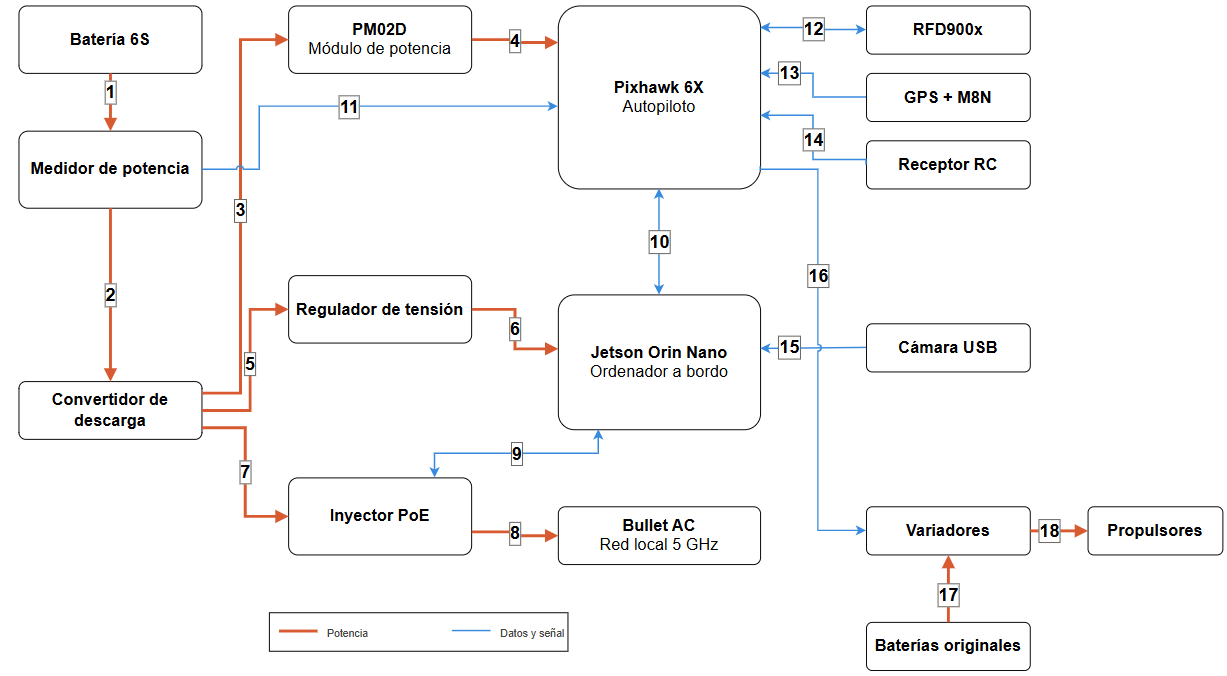
\includegraphics[width=\textwidth]{fig/conexiones.png}
\caption{Esquema de conexiones de alimentación y de datos del hardware embarcado en el USV1. Los números identifican 
cada conexión de la Tabla~\ref{tab:lista_cables}.}
\label{fig:conexionado}
\end{figure}
 
\begin{table}[!htb]
\centering
\caption{Conexiones del hardware embarcado y vehículo en que se instala cada una.}
\label{tab:lista_cables}
\footnotesize
\renewcommand{\arraystretch}{1.15}
\begin{tabularx}{\textwidth}{|>{\raggedright\arraybackslash}p{0.5cm}|>{\raggedright\arraybackslash}p{3.6cm}|>{\raggedright\arraybackslash}p{2.6cm}|>{\raggedright\arraybackslash}X|>{\centering\arraybackslash}p{1cm}|>{\centering\arraybackslash}p{1cm}|}
\hline
\textbf{Nº} & \textbf{Origen → destino} & \textbf{Tipo} & \textbf{Función} & \textbf{USV1} & \textbf{USV2} \\ \hline
1 & Batería 6S → medidor de potencia & Alimentación & Entrada de energía de la carga útil & \checkmark & \checkmark \\ \hline
2 & Medidor de potencia → convertidor de descarga & Alimentación & Medida del consumo total & \checkmark & \checkmark \\ \hline
3 & Convertidor de descarga → PM02D & Alimentación & Rama del autopiloto & \checkmark & \checkmark \\ \hline
4 & PM02D → Pixhawk 6X & Alimentación y datos & Alimentación a 5,2~V y medida de la rama & \checkmark & \checkmark \\ \hline
5 & Convertidor de descarga → regulador de tensión & Alimentación & Rama del ordenador a bordo & \checkmark & -- \\ \hline
6 & Regulador de tensión → Jetson Orin Nano & Alimentación & Alimentación a 18~V & \checkmark & -- \\ \hline
7 & Convertidor de descarga → inyector PoE & Alimentación & Rama del radio & \checkmark & \checkmark \\ \hline
8 & Inyector PoE → Bullet AC & Alimentación y datos (PoE) & Energía y red local en un único cable & \checkmark & \checkmark \\ \hline
9 & Inyector PoE $\leftrightarrow$ Jetson Orin Nano (USV1) o Pixhawk 6X (USV2) & Datos (Ethernet) & Acceso a la red local & \checkmark & \checkmark \\ \hline
10 & Pixhawk 6X $\leftrightarrow$ Jetson Orin Nano & Datos (serie) & Integración del autopiloto con ROS~2 & \checkmark & -- \\ \hline
11 & Medidor de potencia → Pixhawk 6X & Datos (I2C) & Consumo de la carga útil en la telemetría & \checkmark & \checkmark \\ \hline
12 & RFD900x $\leftrightarrow$ Pixhawk 6X & Datos (serie) & Telemetría por el enlace redundante & \checkmark & \checkmark \\ \hline
13 & GPS + M8N → Pixhawk 6X & Datos (serie) & Posición y rumbo & \checkmark & \checkmark \\ \hline
14 & Receptor RC → Pixhawk 6X & Datos & Control manual & \checkmark & \checkmark \\ \hline
15 & Cámara USB → Jetson Orin Nano & Datos y alimentación (USB) & Captura de imágenes & \checkmark & -- \\ \hline
16 & Pixhawk 6X → variadores & Señal (PWM) & Mando de los propulsores & \checkmark & \checkmark \\ \hline
17 & Baterías originales → variadores & Alimentación & Energía de propulsión & \checkmark & \checkmark \\ \hline
18 & Variadores → propulsores & Alimentación & Accionamiento de los propulsores & \checkmark & \checkmark \\ \hline
\end{tabularx}
\end{table}

\newpage
 
La diferencia entre ambos vehículos se concentra en el acceso a la red local. En el USV1, el puerto de datos del 
inyector PoE se conecta a la Jetson, que a su vez se comunica con el autopiloto por el puerto TELEM2, de modo que el 
ordenador a bordo actúa como intermediario entre el autopiloto y el resto del sistema. En el USV2, el mismo puerto se 
conecta directamente al puerto Ethernet del Pixhawk~6X, lo que elimina el ordenador a bordo sin modificar el resto 
del conexionado. La cámara se alimenta y se comunica a través del USB de la Jetson, por lo que no requiere una rama 
de alimentación propia.
 
% ---------------------------------------------------------------------
\subsection{Arquitectura de alimentación y medición de energía}
\label{subsec:alimentacion}
 
La alimentación de cada vehículo se divide en dos dominios independientes. Las baterías originales de la plataforma 
alimentan exclusivamente los variadores y los propulsores, mientras que una batería TATTU 6S de 4500~mAh alimenta toda 
la electrónica de control, percepción y comunicaciones \cite{Cite22}. Esta separación evita que los picos de corriente 
de los propulsores provoquen caídas de tensión capaces de reiniciar el autopiloto, el ordenador a bordo o el radio, 
y mantiene sin modificaciones el sistema de propulsión existente. Ambos dominios se distinguen en la 
Figura~\ref{fig:conexionado}: los cables 1 a 8 corresponden a la carga útil y los cables 17 y 18, a la propulsión.
 
 
La batería de la carga útil proporciona entre 25,2~V a plena carga y unos 19,8~V al final de la descarga, por lo que 
cada rama adapta esa tensión a la de su carga. El autopiloto se alimenta a través del módulo de potencia PM02D, que 
admite baterías de 2S a 12S y entrega 5,2~V regulados con hasta 3~A al autopiloto y a sus periféricos 
\cite{holybro_pm02d}. El Bullet AC se alimenta mediante el inyector PoE pasivo APOE03, que admite entradas de 5 a 
57~V y aplica al cable la misma tensión de entrada, sin negociación \cite{apoe03}; el radio recibe, por tanto, la 
tensión de la batería, próxima a los 24~V de su alimentación PoE pasiva nominal \cite{bulletac}. 
%% PENDIENTE: confirmar el rango de tensión admitido por el Bullet AC (se ha supuesto 20--27 V).
 
La Jetson Orin Nano admite en su entrada de alimentación tensiones de 9 a 20~V \cite{jetson_orin_nano}, inferiores a la 
tensión máxima de la batería, por lo que se alimenta a través del regulador reductor D42V110F18, de 18~V de salida y 
hasta 8~A, con una eficiencia típica superior al 90~\% \cite{pololu_d42v110f18}. La tensión de 18~V se elige por ser la 
más alta dentro del rango de la Jetson que el regulador puede mantener durante la mayor parte de la descarga. Cuando la 
tensión de la batería se aproxima a la de salida, el regulador deja de regular y su salida sigue a la de entrada con 
una pequeña caída; incluso en ese caso la tensión entregada permanece dentro del rango admitido por la Jetson, de modo 
que el ordenador a bordo no limita el aprovechamiento de la batería.
 
El consumo de la carga útil se mide con el medidor I2C-INA-BM, basado en el circuito INA228 de 20~bits, capaz de medir 
tensiones de hasta 85~V y corrientes de hasta 204,8~A \cite{Cite21}. Se instala a la salida de la batería, de modo 
que registra el consumo conjunto de todas las ramas, y se conecta al bus I2C del autopiloto, que lo gestiona como un 
segundo monitor de batería. %% PENDIENTE: confirmar conexión al I2C del autopiloto y punto de medida.

Esta disposición tiene dos ventajas. Por un lado, el consumo de la carga útil forma parte de la telemetría del 
autopiloto, por lo que se registra y se transmite igual en el USV2, que carece de ordenador a bordo. Por otro, el 
autopiloto puede actuar sobre esta medida: el umbral de batería baja de este monitor activa uno de los mecanismos de 
recuperación descritos más adelante en este capítulo.
 
Aunque los dos dominios de alimentación son independientes, las masas de ambos se unen en el autopiloto, ya que las 
señales PWM que gobiernan los variadores necesitan una referencia común.
 
\FloatBarrier
 
\subsection{Presupuesto de potencia y autonomía}
\label{subsec:presupuesto_potencia}
 
La potencia de la carga útil se dimensiona con un criterio conservador: a cada subsistema se le asigna su consumo 
máximo según las hojas de datos y, sobre el total, se aplica un margen de diseño del 25~\%, dentro del intervalo del 
20 al 30~\% habitual para sobredimensionar la alimentación. El autopiloto y sus periféricos (receptor GNSS, radiomódem 
y receptor de radiocontrol) comparten la salida de 5,2~V del módulo de potencia, por lo que se agrupan con el límite de 
corriente de dicho módulo \cite{holybro_pm02d}. Para el ordenador a bordo se considera su modo de máxima potencia, de 
25~W, y se añaden el consumo de la cámara conectada a él y las pérdidas del regulador. La 
Tabla~\ref{tab:presupuesto_potencia} recoge el resultado para cada vehículo.
 
\begin{table}[!htb]
\centering
\caption{Presupuesto de potencia de la carga útil de cada vehículo, con un margen de diseño del 25~\%.}
\label{tab:presupuesto_potencia}
\footnotesize
\renewcommand{\arraystretch}{1.15}
\begin{tabularx}{\textwidth}{|>{\raggedright\arraybackslash}X|>{\raggedright\arraybackslash}p{1.1cm}|>{\raggedright\arraybackslash}p{1.3cm}|>{\raggedright\arraybackslash}p{1.5cm}|>{\raggedright\arraybackslash}p{1.5cm}|}
\hline
\textbf{Subsistema} & \textbf{V (V)} & \textbf{I (mA)} & \textbf{USV1 (W)} & \textbf{USV2 (W)} \\ \hline
Autopiloto y periféricos (Pixhawk 6X, GNSS, RFD900x, receptor RC), límite del módulo PM02D \cite{holybro_pm02d} & 5,2 & 3000 & 15,6 & 15,6 \\ \hline
Red local (Bullet AC) & 24 & 333 & 8,0 & 8,0 \\ \hline
Ordenador a bordo (Jetson Orin Nano, modo de 25~W) & 18 & 1389 & 25,0 & -- \\ \hline
Cámara USB & 5 & 500 & 2,5 & -- \\ \hline
Pérdidas del regulador (rendimiento del 90~\%) & -- & -- & 3,1 & -- \\ \hline
\textbf{Subtotal} & & & \textbf{54,2} & \textbf{23,6} \\ \hline
\textbf{Potencia de diseño (+25~\%)} & & & \textbf{67,7} & \textbf{29,5} \\ \hline
\end{tabularx}
\end{table}
 
La batería almacena unos 100~Wh. Con una profundidad de descarga del 80~\%, que evita descargarla por completo, la 
energía aprovechable es de unos 80~Wh, lo que proporciona una autonomía de diseño de unos 70~min en el USV1 y de unas 
2,7~h en el USV2. Ambas superan con margen la duración mínima de las misiones de prueba, de 30~min en la de desempeño de 
los sensores y de 20~min en la de navegación cooperativa (Sección~\ref{sec:pruebas}); 
en operación típica, con la Jetson en su modo de 15~W, el consumo real es inferior al de diseño y la autonomía aumenta. 
El medidor de potencia permite contrastar estas estimaciones con el consumo medido durante las pruebas.
 
El mismo dimensionamiento sirve para comprobar los elementos de la cadena de alimentación. A la tensión mínima de la 
batería, la potencia de diseño del USV1 supone unos 3,4~A, muy por debajo de la capacidad de descarga de la batería. 
La rama del ordenador a bordo requiere menos de 2~A a 18~V, incluido el margen de diseño, muy por debajo de los 8~A 
del convertidor. Por último, el umbral de batería baja se fija en 21,0~V, equivalente a 3,5~V por celda, de modo que 
la tensión entregada al Bullet AC se mantiene lo más próxima posible a su alimentación nominal de 24~V y el enlace 
principal no se pierde por descarga antes de que el sistema active el retorno.
 
% ---------------------------------------------------------------------
\subsection{Masa añadida} % Al añadir las fotografías: "Masa añadida e integración"
\label{subsec:masa_anadida}
 
La Tabla~\ref{tab:presupuesto_masa} recoge la masa de los componentes que se añaden a cada vehículo, excluidos los que 
ya formaban parte de la plataforma original. Las masas proceden de las hojas de datos y, cuando el fabricante no la 
publica, se indican como estimación; todas se verifican por pesaje en la prueba de M7 de la Sección~\ref{sec:pruebas}.

 
\begin{table}[!htb]
\centering
\caption{Masa de los componentes añadidos a cada vehículo.}
\label{tab:presupuesto_masa}
\footnotesize
\renewcommand{\arraystretch}{1.15}
\begin{tabularx}{\textwidth}{|>{\raggedright\arraybackslash}X|>{\raggedright\arraybackslash}p{2.2cm}|>{\raggedright\arraybackslash}p{2.2cm}|}
\hline
\textbf{Componente} & \textbf{USV1 (g)} & \textbf{USV2 (g)} \\ \hline
Batería TATTU 6S 4500~mAh & 650 & 650 \\ \hline
Bullet AC & 116 & 116 \\ \hline
Jetson Orin Nano (estimación) & 175 & -- \\ \hline
Cámara USB (estimación) & 50 & -- \\ \hline
Inyector PoE APOE03 & 40 & 40 \\ \hline
Convertidor D42V110F18 & 15 & -- \\ \hline
Antena SpiroNET (estimación) & 10 & 10 \\ \hline
Monitor I2C-INA-BM & 4 & 4 \\ \hline
Cableado, conectores y soportes (estimación) & 100 & 80 \\ \hline
\textbf{Total} & \textbf{$\approx$1160} & \textbf{$\approx$900} \\ \hline
\end{tabularx}
\end{table}
 
La masa añadida es de aproximadamente 1,16~kg en el USV1 y 0,90~kg en el USV2, muy por debajo del valor marginal 
de 5~kg de M7 y también del ideal de 4~kg. Sumada a la de la plataforma, de unos 6,2~kg 
(Apéndice~\ref{ap:diagnostico}), la masa total resulta de unos 7,4~kg en el USV1 y 7,1~kg en el USV2, dentro del 
margen de 10 a 12~kg que el grupo recomienda no superar a partir de sus ensayos de lastre. La batería de la 
carga útil representa más de la mitad de la masa añadida en ambos vehículos, por lo que su ubicación en el 
casco es la que más influye en la estabilidad, …por lo que su ubicación en el casco es la que más influye en la 
estabilidad, aspecto que se analiza en la sección de integración física de este capítulo.
%% PENDIENTE: añadir la frase final de la integración física.


% La Figura~\ref{fig:fotos_integracion} muestra el hardware integrado en ambos vehículos. 
%% PENDIENTE: descomentar cuando haya fotografías.
 
%% PENDIENTE: figura comentada hasta disponer de las fotografías.
% --- Figura: fotografías de la integración ----------------------------
% Una fotografía por vehículo con la electrónica montada, con números
% sobre cada componente y leyenda en el pie o en el texto.
% \begin{figure}[!htb]
% \centering
% \begin{subfigure}[t]{0.48\textwidth}
%   \centering
%   % \includegraphics[width=\textwidth]{figuras/foto_usv1.jpg}
%   \fbox{\parbox[c][5cm][c]{0.9\textwidth}{\centering Fotografía pendiente: USV1}}
%   \caption{USV1 (líder).}
%   \label{fig:foto_usv1}
% \end{subfigure}\hfill
% \begin{subfigure}[t]{0.48\textwidth}
%   \centering
%   % \includegraphics[width=\textwidth]{figuras/foto_usv2.jpg}
%   \fbox{\parbox[c][5cm][c]{0.9\textwidth}{\centering Fotografía pendiente: USV2}}
%   \caption{USV2 (seguidor).}
%   \label{fig:foto_usv2}
% \end{subfigure}
% \caption{Hardware embarcado integrado en los dos vehículos. %% PENDIENTE: añadir la leyenda de los números.
% }
% \label{fig:fotos_integracion}
% \end{figure}
 


% =====================================================================
% Capítulo 4 — Sección 4.4: Arquitectura de software (versión 1)
% Claves \cite{...} existentes -> ajustar a las de tu .bib:
%   iniesta2025 [6], albatati2026 [21], cotta2023 [29 o la que uses]
% Claves NUEVAS o por confirmar:
%   jetpack7, usb_cam, vrx (entradas al final)
% =====================================================================
 
\section{Arquitectura de software}
\label{sec:arquitectura_software}
 
Esta sección describe el software que se ejecuta en cada nodo del sistema y cómo se organiza sobre ROS~2. Se presentan 
la pila de software de cada equipo, el grafo de ROS~2 que forman en conjunto, la integración con los autopilotos y la 
cadena de percepción y registro de datos. La lógica de coordinación entre los vehículos, que se apoya en esta 
arquitectura, se detalla en la sección siguiente.
 
% ---------------------------------------------------------------------
\subsection{Pila de software de cada nodo}
\label{subsec:pila_software}
 
La estación base y el ordenador a bordo del USV1 ejecutan Ubuntu 24.04~LTS y ROS~2 Jazzy, de modo que ambos equipos 
comparten la misma distribución de ROS~2 y forman un único grafo sin incompatibilidades entre versiones. En la Jetson 
Orin Nano, este sistema operativo se instala mediante JetPack~7, la versión del paquete de software de NVIDIA basada en 
Ubuntu 24.04 \cite{jetpack7}. Los autopilotos ejecutan ArduPilot Rover 4.7.2. Como la interfaz DDS nativa no 
forma parte del firmware estándar de la placa, el firmware se genera mediante el servicio de compilación 
personalizada de ArduPilot con dicha interfaz habilitada y se instala manualmente en los autopilotos. 
Esta versión admite además la comunicación MAVLink por Ethernet, de modo que un mismo firmware sirve para 
los dos caminos de integración: el USV1 emplea la interfaz DDS y el USV2, MAVLink sobre UDP. La 
Tabla~\ref{tab:pila_software} resume la pila 
de software de cada equipo.

 
\begin{table}[!htb]
\centering
\caption{Pila de software de cada equipo del sistema.}
\label{tab:pila_software}
\footnotesize
\renewcommand{\arraystretch}{1.15}
\begin{tabularx}{\textwidth}{|>{\raggedright\arraybackslash}p{2.8cm}|>{\raggedright\arraybackslash}p{3.4cm}|>{\raggedright\arraybackslash}X|}
\hline
\textbf{Equipo} & \textbf{Base de software} & \textbf{Componentes principales} \\ \hline
Estación base & Ubuntu 24.04~LTS y ROS~2 Jazzy & Coordinador de misión y generador de la ruta del seguidor (desarrollo propio); MAVROS para el USV2; rosbag2; herramientas de visualización de ROS~2; Mission Planner como estación de respaldo \\ \hline
Jetson Orin Nano (USV1) & JetPack~7 (Ubuntu 24.04~LTS) y ROS~2 Jazzy & Agente micro-ROS; controlador de la cámara; detector de obstáculos (desarrollo propio) \\ \hline
Autopilotos (USV1 y USV2) & ArduPilot Rover 4.7.0 o posterior (firmware con DDS habilitado) & Navegación, control de bajo nivel y mecanismos de seguridad; interfaz DDS en el USV1 y MAVLink por Ethernet en el USV2 \\ \hline
\end{tabularx}
\end{table}
 
El reparto de tareas sigue la jerarquía de la Sección~\ref{subsec:arquitectura_informacion}. El control de bajo nivel 
de cada vehículo, es decir, la estimación de estado, el seguimiento de la ruta y el gobierno de los propulsores, queda 
a cargo de ArduPilot, que es la parte validada de la plataforma original \cite{iniesta2025}. El software desarrollado 
en este proyecto se concentra en las tareas de alto nivel que el autopiloto no resuelve por sí solo: la coordinación 
de la flota, la generación de la ruta del seguidor y la detección de obstáculos.
 
\FloatBarrier
 
% ---------------------------------------------------------------------
\subsection{Grafo de ROS 2}
\label{subsec:grafo_ros2}
 
La Figura~\ref{fig:grafo_ros2} representa el grafo de ROS~2 del sistema: sus nodos, los tópicos por los
 que intercambian información y los servicios que emplean. Cada tópico se identifica por la información que 
 transporta y por su tipo de mensaje, todos ellos estándar de ROS~2, lo que permite que las herramientas de 
 registro y de visualización los interpreten sin desarrollo adicional. La información de cada vehículo se publica 
 bajo su propio espacio de nombres, \texttt{/usv1} y \texttt{/usv2}, de modo que el tráfico de ambos permanece 
 separado dentro de un mismo grafo.

 En la Figura~\ref{fig:grafo_ros2}, una flecha de un nodo a un tópico indica que el nodo publica en él y una flecha de un tópico a un 
 nodo, que el nodo se suscribe, y en el caso de los servicios, la flecha distingue al nodo cliente que realiza la petición del 
 nodo servidor que la atiende.

\begin{figure}[!htb]
\centering
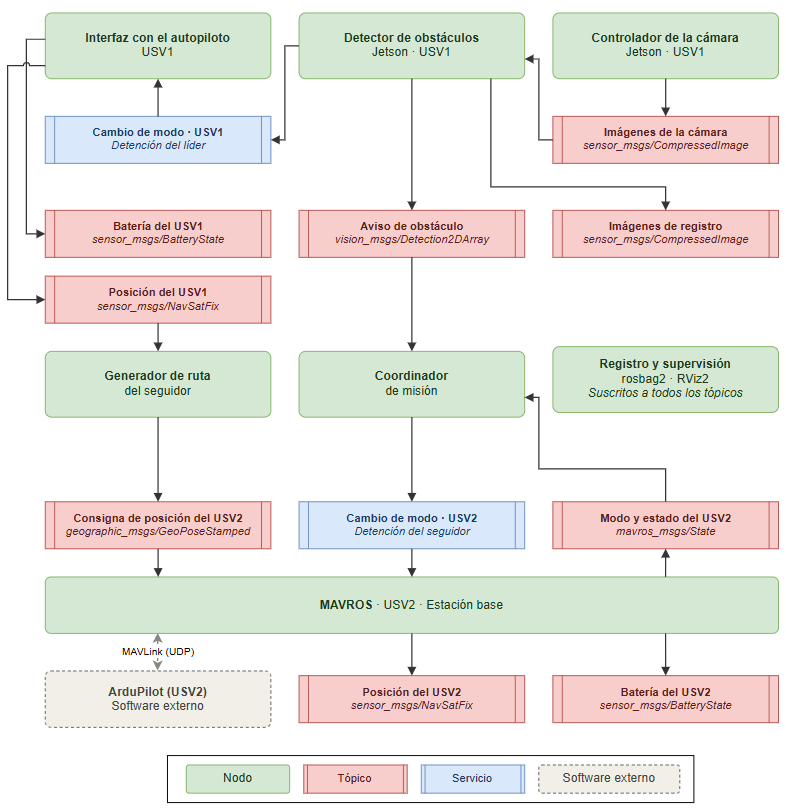
\includegraphics[width=\textwidth]{fig/diagrama_ros2.png}
\caption{Grafo de ROS~2 del sistema multi-USV, con sus nodos, tópicos y servicios.}
\label{fig:grafo_ros2}
\end{figure}

El flujo principal del grafo reproduce el esquema líder--seguidor. La posición del USV1 alimenta al generador de 
ruta, que publica las consignas de posición del USV2, y MAVROS las convierte en órdenes para su autopiloto. En 
paralelo, el detector procesa las imágenes de la cámara y, ante un obstáculo, publica el aviso y solicita al 
autopiloto del USV1 el cambio de modo; el coordinador recibe ese aviso y solicita el mismo cambio para detener al 
USV2. Los tópicos de estado y de batería de ambos vehículos y las imágenes de registro los consumen el registro y 
las herramientas de supervisión.
 
 
% ---------------------------------------------------------------------
\subsection{Integración con los autopilotos}
\label{subsec:integracion_autopilotos}
 
Cada vehículo se integra en el grafo por el camino descrito en la Sección~\ref{subsec:arquitectura_informacion}, y la 
diferencia entre ambos determina también su modo de navegación.
 
En el USV1, la interfaz DDS del autopiloto se habilita en el puerto serie que lo une a la Jetson, donde el agente 
micro-ROS publica su posición y su estado como tópicos de ROS~2 y ofrece servicios para cambiar el modo de navegación 
\cite{albatati2026}. El USV1 navega en modo Auto: antes de la misión, su ruta se carga en el autopiloto como una 
secuencia de \textit{waypoints}, de modo que el líder la recorre de forma autónoma sin depender de consignas en 
tiempo real. Ante un obstáculo, el detector solicita al autopiloto el cambio a un modo de parada a través de la propia 
interfaz DDS, sin intervención de la estación base, lo que reduce el tiempo de reacción del vehículo que abre camino.
 
En el USV2, la interfaz Ethernet del autopiloto se configura para enviar MAVLink sobre UDP a la estación base, donde 
MAVROS lo traduce a ROS~2 bajo el espacio de nombres \texttt{/usv2}. El USV2 navega en modo Guided, que acepta consignas 
de posición enviadas en tiempo real (Sección~\ref{subsec:mavlink_mavros}): el generador de la ruta del seguidor le 
envía, a través de MAVROS, los puntos de la trayectoria ya recorrida por el líder, y el coordinador, la orden de parada 
cuando recibe un aviso de obstáculo.
 
Por último, cada autopiloto recibe un identificador de sistema MAVLink distinto, lo que permite distinguir ambos 
vehículos tanto en MAVROS como en la estación de respaldo.
 
% ---------------------------------------------------------------------
\subsection{Percepción y registro de datos}
\label{subsec:percepcion_registro}
 
La cámara del USV1 se lee en ROS~2 mediante el paquete \texttt{usb\_cam}, disponible para Jazzy, que 
admite el formato MJPEG de las cámaras USB y publica las imágenes comprimidas en JPEG \cite{usb_cam}. Esta 
compresión mantiene el tráfico de imágenes dentro de lo estimado en la Tabla~\ref{tab:demanda_trafico}. 
Sobre estas imágenes se ejecuta el detector de obstáculos, basado en redes neuronales del tipo YOLO, que 
aprovecha la aceleración gráfica de la Jetson y cuya versión concreta se elige según el rendimiento obtenido 
en ella. El Algoritmo~\ref{alg:percepcion} describe el funcionamiento del nodo de percepción.
 
% Traducción al español del entorno algorithmic (puede ir aquí o en el preámbulo)
\floatname{algorithm}{Algoritmo}
\algrenewcommand\algorithmicrequire{\textbf{Entrada:}}
\algrenewcommand\algorithmicwhile{\textbf{mientras}}
\algrenewcommand\algorithmicdo{\textbf{hacer}}
\algrenewcommand\algorithmicif{\textbf{si}}
\algrenewcommand\algorithmicthen{\textbf{entonces}}
\algrenewcommand\algorithmicelse{\textbf{si no}}
\algrenewtext{EndWhile}{\textbf{fin mientras}}
\algrenewtext{EndIf}{\textbf{fin si}}
\algrenewtext{ElsIf}[1]{\textbf{si no, si} #1 \textbf{entonces}}
 
\begin{algorithm}[!htb]
\caption{Percepción y captura de imágenes en el USV1.}
\label{alg:percepcion}
\begin{algorithmic}[1]
\Require imágenes de la cámara y posición del USV1
\Statex \textbf{INICIO}
\While{la misión está activa}
    \State Adquirir una imagen y registrar su instante de captura
    \State Detectar obstáculos en la zona de avance del vehículo
    \If{se detecta un obstáculo}
        \State Solicitar al autopiloto el cambio a modo Hold
        \State Publicar el aviso de obstáculo con la posición y el instante de captura
        \State Publicar la imagen asociada al obstáculo
    \ElsIf{el vehículo está detenido por un obstáculo y no se detecta durante el tiempo de confirmación}
        \State Solicitar al autopiloto el regreso al modo Auto y publicar el fin del aviso
    \ElsIf{ha transcurrido el periodo de captura}
        \State Publicar la imagen para el registro periódico
    \EndIf
\EndWhile
\Statex \textbf{FIN}
\end{algorithmic}
\end{algorithm}
 
El algoritmo atiende tres métricas. Las imágenes se publican de forma periódica con el periodo correspondiente a la 
frecuencia de captura objetivo (M9), y de inmediato cuando se detecta un obstáculo, de modo que todo aviso queda 
documentado con su imagen. Cada imagen conserva su instante de captura, a partir del cual se calcula la latencia de 
adquisición (M3) como el tiempo transcurrido hasta su publicación en ROS~2; como ambos instantes se registran en la 
Jetson, la medida no depende de la sincronización con otros equipos. Por último, la 
publicación continua de los datos de cada sensor permite calcular su disponibilidad durante la misión (M2).
 
El registro de la misión se centraliza en la estación base, donde rosbag2 graba los tópicos de ambos vehículos, 
incluidas las imágenes y los avisos, en un único archivo con una base de tiempo común. Este registro se complementa 
con dos fuentes independientes de la red local: la telemetría que la estación de respaldo recibe por el enlace 
RFD900x, que se conserva en su propio registro, y los registros internos de cada autopiloto. De este modo, una 
pérdida temporal de la red local no interrumpe el registro de la posición ni del estado de los vehículos. Las 
imágenes, que solo pueden transmitirse por la red local, pueden grabarse además en la Jetson cuando se requiera 
conservarlas también durante esas interrupciones.

La telemetría de RPM que exige la Tabla~\ref{tab:necesidades} se resuelve a partir de las salidas PWM que el 
autopiloto envía a cada variador. La plataforma no dispone de sensores de giro en los propulsores, y la consigna 
PWM determina el régimen de cada uno, por lo que se emplea como indicador de ese régimen. Estas salidas forman 
parte de la telemetría MAVLink de ambos autopilotos, que la estación de respaldo recibe por el enlace RFD900x y 
que, en el USV2, MAVROS publica además en ROS~2, y quedan guardadas en los registros internos de cada autopiloto. 
Así, el régimen de los propulsores se transmite en tiempo real y queda registrado en los dos vehículos.


% =====================================================================
% Sección 4.5 — Estrategia de navegación cooperativa
% Requiere los paquetes algorithm/algpseudocode ya cargados para el Algoritmo 1.
% Figura 4.9: sustituir la ruta de \includegraphics por la de tu imagen.
% Claves \cite{...} -> ajustar a tu .bib:
%   jin2023 = [16] (círculo de aceptación), ublox_neo_m8 = [29]
% Etiquetas \ref{...} marcadas con % AJUSTAR -> cambiar por las tuyas.
% =====================================================================
\section{Estrategia de navegación cooperativa}
\label{sec:navegacion_cooperativa}

Esta sección desarrolla la lógica con la que la estación base coordina a los dos vehículos durante la fase de 
ejecución de la Figura~\ref{fig:flujo_ejecucion}. 

Responde a la necesidad de coordinar dos USV mediante navegación por waypoints como primera demostración de 
operación multivehículo (Tabla~\ref{tab:necesidades}) y a las métricas que la verifican en campo: el error de 
trayectoria (M4), la latencia de comunicación (M5) y la tasa de éxito de misión (M6). Esta lógica reside en los 
dos nodos de la estación base de la Figura~\ref{fig:grafo_ros2}, el coordinador de misión y el generador de ruta 
del seguidor, mientras que el seguimiento de cada tramo lo resuelve el autopiloto de cada vehículo 
(Sección~\ref{subsec:integracion_autopilotos}).

% ---------------------------------------------------------------------
\subsection{Planificación de la misión}
\label{subsec:planificacion_mision}

La misión se define en la preparación (Figura~\ref{fig:flujo_prep_cierre}a) como una lista ordenada de puntos de 
muestreo en coordenadas geográficas, que el operador elabora sobre el mapa de la zona y que el coordinador lee 
desde un archivo. Esa misma lista constituye la ruta del líder, que se carga en su autopiloto antes de la misión, y la del 
seguidor, que la recorre con retraso. Así, ambos vehículos comparten la numeración de los puntos y cada punto 
se muestrea dos veces en instantes distintos. Se denomina tramo al segmento recto entre dos puntos consecutivos, 
que es la referencia sobre la que se calcula el error transversal (Sección~\ref{subsec:guiado_waypoints}). 

Al final de la ruta del líder se añade un punto de espera, situado más allá del último punto de muestreo y fuera 
de la ruta del seguidor. Este punto no forma parte de los ensayos de M6; su función es que el líder despeje el 
último punto de muestreo antes de que el seguidor se dirija hacia él, de modo que ambos vehículos nunca coinciden 
en un mismo punto.

La misión se completa con los parámetros de la Tabla~\ref{tab:parametros_mision}, comunes a ambos vehículos. El 
más directamente ligado a las métricas es el radio de aceptación, que define cuándo se considera alcanzado un 
punto \cite{jin2025}. Se fija en 2~m, del orden de la incertidumbre del receptor GNSS \cite{Cite29} y del 
valor marginal de M4: un radio menor exige una precisión que el posicionamiento no garantiza y provoca maniobras 
de corrección alrededor de cada punto, mientras que uno mayor resta representatividad al punto de muestreo. La 
distancia entre puntos consecutivos se elige varias veces mayor que ese radio, para que cada tramo incluya un 
recorrido recto en el que el vehículo se estabilice sobre la línea. La velocidad de crucero se fija en 1,0~m/s, 
por debajo de la velocidad sostenida de 1,2 a 1,3~m/s que alcanza la plataforma, de modo que el autopiloto 
dispone de margen de empuje para corregir el rumbo frente al viento o la corriente, y es la misma en ambos 
vehículos para que el seguidor no alcance al líder por una diferencia de velocidad. Los demás parámetros se 
justifican en las secciones siguientes.

\begin{table}[!htb]
\centering
\caption{Parámetros de diseño de la misión cooperativa.}
\label{tab:parametros_mision}
\small
\begin{tabularx}{\textwidth}{|>{\raggedright\arraybackslash}p{3.3cm}|>{\raggedright\arraybackslash}p{2.6cm}|>{\raggedright\arraybackslash}X|>{\centering\arraybackslash}p{1.4cm}|}
\hline
\textbf{Parámetro} & \textbf{Valor de diseño} & \textbf{Criterio} & \textbf{Métrica} \\ \hline
Velocidad de crucero & 1,0~m/s en ambos USV & Inferior a la velocidad sostenida de la plataforma (Apéndice~\ref{ap:diagnostico}) e igual en ambos vehículos & M4, M6 \\ \hline
Radio de aceptación & 2~m & Incertidumbre del GNSS y valor marginal de M4 & M4, M6 \\ \hline
Distancia entre puntos & $\geq$10~m & Tramo recto suficiente para estabilizarse sobre la línea & M4 \\ \hline
Retraso del seguidor & 1 tramo & El seguidor solo navega por zonas ya inspeccionadas & M6 \\ \hline
Separación mínima & 10~m & Incertidumbre de ambos GNSS, frenado y retardo de coordinación & M5 \\ \hline
Tiempo de confirmación & 3~s & Evita reanudar la marcha por una detección perdida & M6 \\ \hline
Tiempo máximo de espera & 60~s & Un obstáculo persistente se gestiona como fallo & M10 \\ \hline
\end{tabularx}
\end{table}

% ---------------------------------------------------------------------
\subsection{Generación de la ruta del seguidor}
\label{subsec:ruta_seguidor}

El seguidor no recibe la ruta completa al inicio, sino punto a punto, a medida que el líder la inspecciona. 
El generador de ruta compara la posición del USV1 con los puntos de la misión y, cada vez que el líder alcanza 
un punto, habilita para el seguidor el punto anterior. De este modo, el USV2 solo se dirige a puntos que el 
líder ya ha superado, con una separación mínima de un tramo. 

Cuando el USV2 alcanza su punto, el generador le envía el siguiente punto habilitado como consigna de posición 
en modo Guided; si no hay ninguno, el USV2 permanece detenido en el punto alcanzado hasta que el líder avance. 
Así, cualquier retraso o detención del líder se traslada al seguidor sin necesidad de órdenes adicionales, y el 
último punto de muestreo se habilita cuando el líder alcanza el punto de espera.

La separación de un tramo garantiza que el seguidor navegue por zonas ya inspeccionadas, pero no impide por sí 
sola que se aproxime al líder, por ejemplo cuando este se detiene poco después de un punto. Por ello, el 
coordinador vigila también la distancia entre ambos vehículos, calculada a partir de sus posiciones, y detiene 
al USV2 en modo Hold si es menor que una separación mínima. La separación mínima, de 10~m, cubre la suma de las 
incertidumbres de posición de los dos receptores, del orden de 2~m cada una, la distancia de frenado del seguidor 
y la que recorre durante el retardo máximo admitido para la coordinación (M5), que a la velocidad de crucero 
equivale a 1~m por cada segundo de retardo.

El Algoritmo~\ref{alg:coordinacion} reúne estas reglas con la detención ante obstáculos y la gestión de fallos, 
en el orden de prioridad con que las evalúa el coordinador: primero los fallos, después las condiciones de 
detención del seguidor y, por último, su avance normal.

\begin{algorithm}[!htb]
\caption{Coordinación de la flota en la estación base.}
\label{alg:coordinacion}
\begin{algorithmic}[1]
\Require ruta de la misión, posición y estado de ambos USV
\Statex \textbf{INICIO}
\State Asignar el modo Auto al USV1 y el modo Guided al USV2
\While{el USV2 no ha completado la ruta}
    \If{se detecta un fallo en algún vehículo}
        \State Detener la flota y ejecutar la recuperación (Sección~\ref{sec:recuperacion})
    \ElsIf{hay un aviso de obstáculo o la separación es insuficiente}
        \State Solicitar el modo Hold al USV2
    \Else
        \State Devolver el USV2 al modo Guided si estaba detenido
        \If{el USV1 alcanza un nuevo punto}
            \State Habilitar para el USV2 el punto anterior de la ruta
        \EndIf
        \If{el USV2 alcanza su punto y hay otro punto habilitado}
            \State Enviar al USV2 el siguiente punto habilitado
        \EndIf
    \EndIf
\EndWhile
\State Ordenar a ambos vehículos el retorno al punto de partida
\Statex \textbf{FIN}
\end{algorithmic}
\end{algorithm}

Como resultado, el modo de cada autopiloto refleja en todo momento la situación de la misión. La 
Tabla~\ref{tab:modos_mision} resume estas combinaciones y el nodo que solicita cada cambio, lo que permite al 
operador interpretar el estado de la flota a partir de los modos que publican ambos vehículos.

\begin{table}[!htb]
\centering
\caption{Modos de los autopilotos según la situación de la misión.}
\label{tab:modos_mision}
\small
\begin{tabularx}{\textwidth}{|>{\raggedright\arraybackslash}p{3.6cm}|>{\raggedright\arraybackslash}p{2.5cm}|>{\raggedright\arraybackslash}p{2.5cm}|>{\raggedright\arraybackslash}X|}
\hline
\textbf{Situación} & \textbf{USV1 (líder)} & \textbf{USV2 (seguidor)} & \textbf{Cambio solicitado por} \\ \hline
Inicio de la ejecución & Auto & Guided & Coordinador \\ \hline
Avance normal & Auto & Guided, en avance o en espera & -- \\ \hline
Separación insuficiente & Auto & Hold & Coordinador \\ \hline
Obstáculo detectado & Hold & Hold & Detector (USV1) y coordinador (USV2) \\ \hline
Paso despejado & Auto & Guided & Detector (USV1) y coordinador (USV2) \\ \hline
Fin de la ruta del líder & Hold, en el punto de espera & Guided & Autopiloto del USV1 \\ \hline
Fallo en algún vehículo & Hold o acción de seguridad & Hold o acción de seguridad & Coordinador o autopiloto (Sección~\ref{sec:recuperacion}) \\ \hline
Cierre de la misión & RTL & RTL & Coordinador \\ \hline
\end{tabularx}
\end{table}

% ---------------------------------------------------------------------
\subsection{Detención y reanudación ante obstáculos}
\label{subsec:detencion_obstaculos}

La detención ante un obstáculo se resuelve en dos niveles con distinta latencia. En el USV1, el detector solicita 
el modo Hold directamente a su autopiloto (Algoritmo~\ref{alg:percepcion}), sin pasar por la estación base, por 
lo que la reacción del líder no depende del enlace. El aviso llega después al coordinador, que solicita el mismo 
modo al USV2. Esta segunda detención sí atraviesa el enlace, y su retardo, acotado por M5, no compromete la 
seguridad del seguidor, que se encuentra al menos un tramo por detrás del obstáculo cuando recibe la orden.

La reanudación es automática. El detector considera el paso despejado cuando deja de detectar el obstáculo 
durante un tiempo de confirmación, que evita reanudar la marcha por una detección perdida en una sola imagen. 
En ese momento devuelve el USV1 al modo Auto, en el que el autopiloto retoma la ruta desde el punto pendiente, 
y publica el fin del aviso; al recibirlo, el coordinador devuelve el USV2 al modo Guided y le reenvía su punto 
asignado. Si el obstáculo persiste más allá de un tiempo máximo de espera, la detención deja de tratarse como 
una incidencia de la navegación y se gestiona como un fallo, con la flota detenida a la espera del operador 
(Sección~\ref{sec:recuperacion}).

% ---------------------------------------------------------------------
\subsection{Medición del desempeño cooperativo}
\label{subsec:medicion_desempeno}

El diseño anterior determina cómo se obtienen en campo las métricas de la validación del sistema completo 
(Sección~\ref{subsec:pruebas_sistema}), todas a partir del registro centralizado de la estación base 
(Sección~\ref{subsec:percepcion_registro}). El error de trayectoria (M4) se calcula, para cada vehículo y cada muestra de la posición estimada por su 
autopiloto, como la distancia perpendicular a la recta del tramo que recorre en ese instante 
(Ecuación~\ref{eq:error_transversal}). Como ambos vehículos recorren los mismos tramos, el cálculo es idéntico para el líder y para el seguidor, y solo 
se excluyen los intervalos en modo Hold, en los que el vehículo está detenido y no sigue ningún tramo.

La latencia de comunicación (M5) se estima como la mitad del tiempo de ida y vuelta de un mensaje entre la 
estación base y cada vehículo, lo que evita depender de la sincronización de sus relojes. En el USV1, un nodo 
auxiliar de la estación base envía cada segundo un mensaje con su instante de emisión, que la Jetson devuelve 
de inmediato; este nodo solo se ejecuta durante las pruebas, por lo que no figura en el grafo de la 
Figura~\ref{fig:grafo_ros2}. En el USV2, que carece de ordenador, se emplea el intercambio de mensajes de 
sincronización temporal de MAVLink, en el que el autopiloto responde a cada mensaje enviado desde la estación base, 
que MAVROS emite con la misma frecuencia de 1~Hz. Como complemento, el registro permite medir el tiempo de 
reacción de la flota ante un obstáculo, desde 
que el aviso llega a la estación base hasta que el USV2 confirma el modo Hold, con ambos instantes tomados con 
el reloj de la base.

Por último, la tasa de éxito de misión (M6) se obtiene de los puntos que el coordinador registra como alcanzados 
por cada vehículo, es decir, aquellos en cuyo radio de aceptación ha entrado y en los que se ha registrado el 
evento de muestreo, con la posición y el instante de llegada en ambos vehículos y, en el USV1, la imagen 
asociada. Al cierre de la misión, cada punto de muestreo alcanzado o no alcanzado se contabiliza como un ensayo,  
sin incluir el punto de espera del líder, y la misión se evalúa frente a los criterios de éxito definidos en la 
preparación (Figura~\ref{fig:flujo_prep_cierre}b).

% =====================================================================
% Sección 4.6 — Mecanismos de recuperación ante fallos
% Claves \cite{...} -> ajustar a tu .bib:
%   iniesta2025 = [6], ref13 = [13], ref17 = [17]
% Etiquetas \ref{...} marcadas con % AJUSTAR -> cambiar por las tuyas.
% =====================================================================
\section{Mecanismos de recuperación ante fallos}
\label{sec:recuperacion}

Esta sección desarrolla el subproceso de recuperación de la Figura~\ref{fig:flujo_ejecucion}, al que remiten tanto la ejecución de cada vehículo como el coordinador (Algoritmo~\ref{alg:coordinacion}). % AJUSTAR
Responde a la necesidad de contar con mecanismos redundantes para recuperar la embarcación ante fallos (Tabla~\ref{tab:necesidades}), de importancia 5, y a la métrica que la verifica, el número de mecanismos de recuperación (M10), con un valor marginal de tres y un valor ideal de cuatro. El diseño aplica a la flota los mecanismos de seguridad descritos en la Sección~\ref{subsec:failsafe} y sigue un criterio común: ante cualquier fallo, la flota se detiene y la decisión de continuar corresponde al operador. Un vehículo solo actúa por sí mismo, regresando al punto de partida, cuando queda aislado de ambas estaciones o cuando su batería alcanza el umbral de descarga.

% ---------------------------------------------------------------------
\subsection{Mecanismos del sistema}
\label{subsec:mecanismos_sistema}

El sistema dispone de cuatro mecanismos de recuperación, resumidos en la Tabla~\ref{tab:mecanismos_recuperacion}. Cada uno se apoya en un canal o en un elemento distinto, de modo que el fallo de uno no inutiliza a los demás.

El primero es el enlace redundante con la estación de respaldo. El enlace RFD900x permanece activo en paralelo a la red local durante toda la misión (Sección~\ref{subsec:enlace_redundante}) y lleva la telemetría MAVLink de ambos vehículos a la estación de respaldo, desde la que el operador puede cambiar el modo de cualquiera de ellos. Así, la pérdida de la red local no supone la pérdida de la supervisión ni del mando de la flota. % AJUSTAR

El segundo son las acciones de seguridad del autopiloto, que vigila de forma continua su batería y la calidad de su estimación de posición y ejecuta una acción automática al detectar una condición anómala \cite{kumar2025} \cite{aliane2026}. Cuando la tensión de la batería de la carga útil baja del umbral de 21,0~V fijado en la Sección~\ref{subsec:presupuesto_potencia}, el vehículo regresa al punto de partida en modo RTL, porque la energía restante debe reservarse para el retorno. Ante una degradación del posicionamiento, en cambio, pasa a Hold, ya que con una posición poco fiable el retorno autónomo tampoco es seguro. En el USV2, el autopiloto vigila además la comunicación con las estaciones a partir de la telemetría MAVLink que recibe por los dos enlaces, desde MAVROS por la red local y desde la estación de respaldo por el RFD900x, y ejecuta RTL solo cuando deja de recibirla por ambos. % AJUSTAR

El tercero es la supervisión que ejercen el coordinador y el ordenador a bordo. El coordinador vigila la llegada de los tópicos de ambos vehículos y, si deja de recibir los de uno de ellos, detiene al otro en modo Hold, de modo que la flota no continúa con un vehículo fuera de servicio. En el USV1, el enlace con la estación base no llega al autopiloto como telemetría MAVLink, sino a través del ordenador a bordo. Por ello, es la Jetson la que vigila la red local, mediante un mensaje periódico de presencia que publica el coordinador: si deja de recibirlo durante 5~s, solicita el modo Hold a su autopiloto y, si el enlace no se recupera en 30~s, el modo RTL. Durante ese intervalo, el operador conserva el mando del vehículo a través de la estación de respaldo. De este modo, ambos vehículos responden igual a la pérdida de comunicación, aunque en cada uno la resuelva un elemento distinto.

El cuarto es la recuperación manual. Mediante un conmutador de la emisora de radiocontrol, el operador puede pasar el vehículo al modo Manual en cualquier momento, con prioridad sobre cualquier modo automático \cite{iniesta2025}. Es el último nivel de recuperación y el único que no depende de ningún elemento del sistema autónomo, por lo que cubre también los fallos del ordenador a bordo y de la estación base.

\begin{table}[!htb]
\centering
\caption{Mecanismos de recuperación del sistema multi-USV.}
\label{tab:mecanismos_recuperacion}
\small
\begin{tabularx}{\textwidth}{|>{\raggedright\arraybackslash}p{4.2cm}|>{\raggedright\arraybackslash}p{3.8cm}|>{\raggedright\arraybackslash}X|}
\hline
\textbf{Mecanismo} & \textbf{Elemento que lo ejecuta} & \textbf{Fallos que cubre} \\ \hline
Enlace redundante y estación de respaldo & RFD900x y Mission Planner & Pérdida de la red local \\ \hline
Acciones de seguridad del autopiloto & Autopiloto de cada USV & Batería baja, degradación del posicionamiento y aislamiento del USV2 \\ \hline
Supervisión del coordinador y del ordenador a bordo & Coordinador y Jetson del USV1 & Fallo de un vehículo, pérdida de la red local y aislamiento del USV1 \\ \hline
Recuperación manual & Emisora de radiocontrol & Cualquier fallo, incluidos los del ordenador a bordo y la estación base \\ \hline
\end{tabularx}
\end{table}

% ---------------------------------------------------------------------
\subsection{Respuesta ante cada fallo}
\label{subsec:respuesta_fallos}

La Tabla~\ref{tab:respuesta_fallos} recoge la respuesta del sistema a cada fallo considerado, distinguiendo entre el vehículo afectado y el resto de la flota. Los fallos corresponden a los del concepto de operación (Sección~\ref{subsec:concepto_operacion}), es decir, la pérdida de un enlace, la falta de energía y la degradación del posicionamiento, a los que se añaden el fallo del ordenador a bordo y la persistencia de un obstáculo. % AJUSTAR

\begin{table}[!htb]
\centering
\caption{Respuesta del sistema ante cada fallo.}
\label{tab:respuesta_fallos}
\small
\begin{tabularx}{\textwidth}{|>{\raggedright\arraybackslash}p{3.1cm}|>{\raggedright\arraybackslash}p{3.0cm}|>{\raggedright\arraybackslash}X|>{\raggedright\arraybackslash}p{2.8cm}|}
\hline
\textbf{Fallo} & \textbf{Detección} & \textbf{Vehículo afectado} & \textbf{Resto de la flota} \\ \hline
Pérdida de la red local & Coordinador y, en el USV1, la Jetson & USV1: Hold y RTL tras 30~s. USV2: se detiene al alcanzar su punto & Hold \\ \hline
Pérdida del enlace RFD900x & Estación de respaldo & Continúa la misión & Continúa; aviso al operador \\ \hline
Pérdida de ambos enlaces & Jetson (USV1) y autopiloto (USV2) & RTL & Hold \\ \hline
Batería baja & Autopiloto, con el medidor de potencia & RTL & Hold \\ \hline
Degradación del posicionamiento & Autopiloto & Hold & Hold \\ \hline
Fallo del ordenador a bordo del USV1 & Coordinador, por la pérdida de sus tópicos & Hold o RTL desde la estación de respaldo, o modo Manual & Hold \\ \hline
Obstáculo persistente & Detector, tras el tiempo máximo de espera & Hold & Hold \\ \hline
\end{tabularx}
\end{table}

La pérdida del enlace RFD900x es el único fallo que no detiene la flota, porque la misión se coordina por la red local y el enlace de respaldo solo se necesita cuando esta falla; basta con avisar al operador de que el sistema ha perdido su redundancia. En el resto de los casos, el coordinador detiene al vehículo que sigue operativo, porque el USV2 depende de la percepción del líder y continuar con un solo vehículo deja de ser una misión cooperativa.

El fallo del ordenador a bordo del USV1 muestra la necesidad de los mecanismos que no dependen del sistema autónomo. Si la Jetson deja de funcionar, el USV1 pierde a la vez la percepción y la conexión con la estación base, pero su autopiloto continúa en modo Auto, ya que no recibe ninguna orden de detención. El coordinador lo detecta por la desaparición de sus tópicos y detiene al USV2, mientras que el USV1 se recupera desde la estación de respaldo, que conserva su mando a través del RFD900x, o mediante el control manual. Un fallo del ordenador de la estación base se gestiona del mismo modo que la pérdida de la red local o, si también deja fuera de servicio a la estación de respaldo, que la pérdida de ambos enlaces.

% ---------------------------------------------------------------------
\subsection{Reanudación y verificación}
\label{subsec:reanudacion_fallos}

A diferencia de la detención ante un obstáculo (Sección~\ref{subsec:detencion_obstaculos}), la reanudación tras un fallo no es automática. Una vez restablecida la condición, el operador decide desde la estación base entre reanudar la misión, en cuyo caso el coordinador devuelve a cada vehículo a su modo de ejecución y el seguidor recibe de nuevo su punto asignado; finalizarla, ordenando el retorno de la flota, o tomar el control manual del vehículo afectado. Si un vehículo ya ha ejecutado RTL, la misión solo puede finalizarse, y los puntos de muestreo que quedan sin alcanzar se contabilizan como no alcanzados en M6.

Con estos cuatro mecanismos, el diseño alcanza el valor ideal de M10. La Prueba~4 de la Sección~\ref{subsec:pruebas_unitarias} los verifica provocando, de uno en uno, los fallos de la Tabla~\ref{tab:respuesta_fallos} que pueden reproducirse de forma segura. Se desconectan por separado la red local y el RFD900x, después ambos a la vez, y se interrumpe la señal del receptor GNSS. En cada caso se comprueba que la supervisión se mantiene por los canales restantes o que se ejecuta la acción correspondiente. La acción de batería baja se comprueba elevando temporalmente el umbral por encima de la tensión de la batería, y la recuperación manual, conmutando la emisora durante una misión. % AJUSTAR